\UseRawInputEncoding
%% R4Tun — Automation in Construction (cas-dc double-column template)

\documentclass[a4paper,fleqn]{cas-dc}

\usepackage[numbers]{natbib}
\usepackage{booktabs}
\usepackage{multirow}
\usepackage{amsmath}
\usepackage{algorithm}
\usepackage{algpseudocode}
\usepackage{graphicx}
\usepackage[dvipsnames,table]{xcolor}
% Better line breaks for long URLs (esp. in two-column bibliographies)
\usepackage{xurl}
\usepackage{hyperref}
% Clever cross-references (\cref, \Cref). Must be loaded after hyperref.
\usepackage[nameinlink,noabbrev]{cleveref}
\usepackage{placeins}
\usepackage{caption}
\usepackage{balance}
\usepackage[normalem]{ulem}
\usepackage{float}
% Highlight review changes with soul \hl (yellow); load after ulem.
%\usepackage{dblfloatfix}
\usepackage{soul}
\sethlcolor{yellow}
\let\texthl\hl
\renewcommand{\hl}[1]{\ifmmode\colorbox{yellow}{\ensuremath{#1}}\else\texthl{#1}\fi}
\soulregister\cite7
\soulregister\ref7
\soulregister\pageref7
\soulregister\cref7
\soulregister\Cref7
\soulregister\eqref7
\usepackage[most]{tcolorbox} % for section-wide / float highlighting
\usepackage{listings}
\lstset{
  basicstyle=\ttfamily\footnotesize,
  breaklines=true,
  columns=fullflexible,
  frame=single,
  framesep=4pt,
  xleftmargin=0.5em,
  xrightmargin=0.5em,
  aboveskip=0.6em,
  belowskip=0.6em,
}
% Yellow frame for new tables / appendix blocks (soul \hl cannot wrap floats).
\newtcolorbox{hlbox}{
  colback=yellow!25,
  colframe=yellow!60!orange,
  boxrule=0.4pt,
  left=2pt,right=2pt,top=2pt,bottom=2pt,
  before skip=0.6em,
  after skip=0.6em,
}

\providecommand{\printorcid}{}
\providecommand{\printfacebook}{}
\providecommand{\printtwitter}{}
\providecommand{\printlinkedin}{}
\providecommand{\printgplus}{}
\providecommand{\printinstagram}{}
\providecommand{\printemails}{}
\providecommand{\printurls}{}
\usepackage{lineno} % line numbers
% \linenumbers % (enabled below after \maketitle)

\begin{document}
\let\WriteBookmarks\relax
\def\floatpagepagefraction{1}
\def\textpagefraction{.001}



% ────────────────────────────── Front matter ──────────────────────────────

\shorttitle{Proxy-guided quality control for tunnel-lining segmentation from point clouds}
\shortauthors{X.\ Tao et~al.}

\title[mode=title]{\texorpdfstring{Proxy-guided quality control for tunnel-lining segmentation from point clouds}{Proxy-guided quality control for tunnel-lining segmentation from point clouds}}

\author[1]{Xinghui Tao}
\credit{Conceptualization, Methodology, Software, Writing -- original draft}

\author[2]{Zehao Ye}


\author[1]{Guangming Wang}
\cormark[1]
\ead{gw462@cam.ac.uk}
\credit{Supervision, Writing -- review \& editing}

\author[2]{Jelena Nini\'{c}}
\credit{Supervision, Writing -- review \& editing}

\author[1]{Brian Sheil}
\credit{Supervision, Funding acquisition, Project administration, Writing -- review \& editing}

\cortext[cor1]{Corresponding author}

\affiliation[1]{organization={Construction Engineering, University of Cambridge},
    addressline={Trumpington Street},
    city={Cambridge},
    postcode={CB2 1PZ},
    country={United Kingdom}}

\affiliation[2]{organization={Department of Engineering, Durham University},
    addressline={Stockton Road},
    city={Durham},
    postcode={DH1 3LE},
    country={United Kingdom}}

% ─── Abstract ─────────────────────────────────────────────────────────────


\begin{abstract}
Point-cloud segmentation of segmental tunnel linings supports automated inspection, but settings tuned for one tunnel can degrade on another, and without deployment ground-truth (GT) labels the new output is hard to verify and refine. Proxy4Tun estimates segmentation accuracy from intermediate pipeline metrics and uses the estimate for deployment-time quality assessment and candidate selection during self-refinement, without deployment labels. Calibration requires one labelled subset and one expert reference per lining family. Across the three Seg2Tunnel families, bounded sampling and uncertainty-guided Bayesian exploration produce 120 calibration runs, from which a four-feature ridge-regression proxy combining preprocessing-quality and structure-coherency metrics is frozen. \hl{The compact proxy includes assumed-line count as a structural feature.} On 54 held-out runs from 27 held-out subsets, the frozen proxy achieves Spearman $\rho=\hl{0.789}$ and MAE $0.106$, and ranks the reference above its degraded counterpart in all 27 pairs. Self-refinement is then tested against a demanding baseline: the expert-reference settings (mean mIoU $0.762$ over 27 subsets). Under an identical three-attempt budget and the same proxy-based selection rule, refinement proposed by three large language models (GPT-5.6, Fable-5.1, Gemini-3.8) raises the selected mean to $0.765$, $0.774$, and $\hl{0.787}$, whereas adaptive-random proposals \hl{reach $0.754$}. LLM proposals preserve accuracy far better: 7--19\% of them lose more than $0.05$ mIoU, against 62\% for adaptive-random proposals. \hl{Gains concentrate in six subsets where the expert-reference baseline starts below mIoU 0.7. A separate STSD subset provides initial external-control evidence.} Proxy4Tun is presented as an exploratory quality control (QC) framework rather than a certified verifier of segmentation accuracy.
\end{abstract}


% ─── Highlights ───────────────────────────────────────────────────────────

\begin{highlights}
\item Proxy4Tun supports segmentation quality control without deployment labels.
\item Calibration uses one labelled subset and one expert reference per lining family.
\item The frozen proxy correctly ranks all 27 reference--degradation pairs.
\item LLM proposals better preserve accuracy than adaptive-random proposals.
\item Refinement gains concentrate where expert settings produce lower initial accuracy.
\end{highlights}

% ─── Keywords ─────────────────────────────────────────────────────────────
\begin{keywords}
Segmental tunnel lining \sep Point cloud segmentation \sep Deployment quality control \sep Label-free proxy \sep self-refinement \sep LLM
\end{keywords}
\date{\today}

\maketitle
% \linenumbers % disabled for now

\smallskip
% ─────────────────────────────────────────────────────────────────────────

\section{Introduction}
\label{sec:intro}

Regular inspection of segmental tunnel linings supports structural health assessment and long-term operational safety. However, large tunnel networks and restricted access make manual inspection resource-intensive, motivating cost-effective data collection and analysis~\cite{attard2018,montero2015,strauss2020sensing}. As one of the main data-collection methods, laser scanning can quickly capture the lining surface as a 3D point cloud~\cite{huang2021bim,sjolander2023towards,weidner2024generalized}, and segmenting the lining into individual segments enables downstream automated tasks such as predictive-maintenance workflows.

\begin{figure*}[t]
\centering
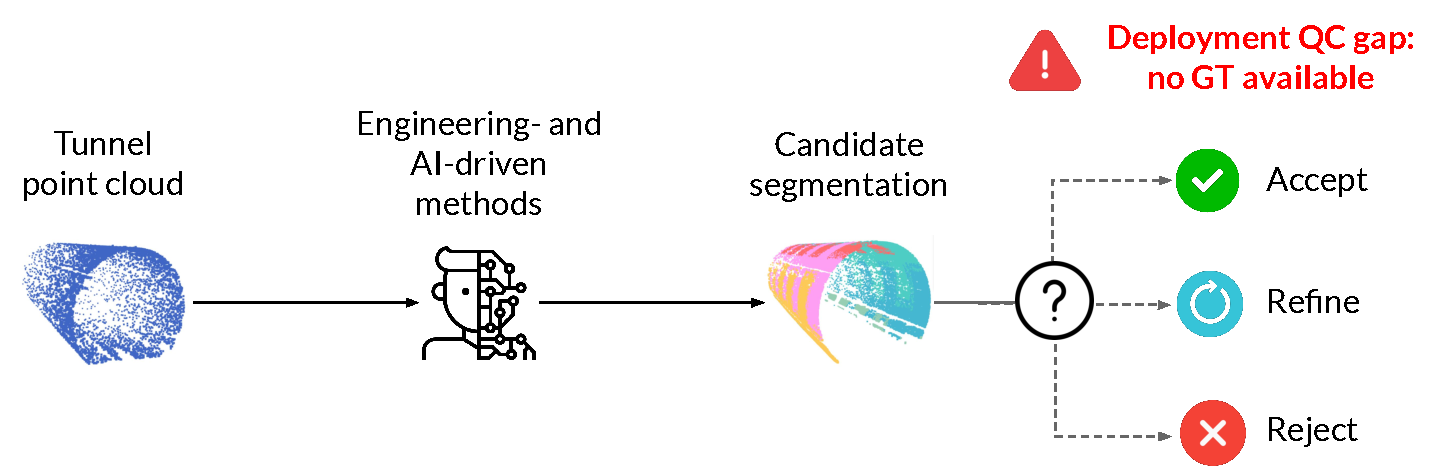
\includegraphics[width=0.8\textwidth]{figs/motivation.pdf}
\caption{Deployment QC problem: segmentation methods produce candidate outputs, but practitioners still need to decide whether to accept, refine, or flag each result without new GT labels.}
\label{fig:deployment_qc_gap}
\end{figure*}

Several tunnel-lining segmentation methods now exist, but parameters tuned for one tunnel can degrade on another as lining geometry, joint layout, occlusion, and scan quality vary. Engineer-designed geometric pipelines use hand-crafted rules and thresholds with interpretable checks, but changes in geometry or scan quality can require manual tuning or redesign~\cite{huang2021bim,weidner2024generalized,wang2025automated}. Supervised models can be retrained on labelled data and may provide confidence or uncertainty scores, but these scores must be checked against actual accuracy before they can support QC on new scans~\cite{su2024review,cha2024deep}. Foundation-model pipelines can reduce per-project annotation and support adaptation through prompts and preprocessing parameters~\cite{bommasani2021foundation,kirillov2023sam,ye2024sam}, however, without deployment labels, segmentation quality remains difficult to assess, limiting refinement because it is unclear whether a proposed change improves or degrades accuracy.

This gap matters in practice for two reasons. First, an undetected segmentation failure can propagate into downstream metrics, while a fixed configuration that provides no quality signal leaves engineers to check each new output. Second, without GT labels, the benefit of a parameter change cannot be directly confirmed, and maximising an indirect quality score can worsen actual segmentation accuracy. Practitioners therefore need an empirically evaluated quality signal to support deployment-time decisions: accept the output, refine it, or flag it for human review (Fig.~\ref{fig:deployment_qc_gap}).

Previous studies show that segmentation accuracy can be estimated without case-specific GT labels. In medical imaging, for example, quality estimators learn from labelled development data or assess new outputs using labelled reference collections~\cite{valindria2017rca,robinson2018segmentationQuality,fournel2021segmentationQC}. However, it remains unclear how well these approaches transfer to tunnel point-cloud pipelines, where annotations are limited and parameter settings often depend on lining geometry. This motivates our central research question: \emph{Can intermediate metrics from a tunnel-segmentation pipeline support accuracy estimation and parameter self-refinement on \hl{held-out tunnel sections} without new GT labels?}

We therefore propose Proxy4Tun, a QC framework that estimates segmentation accuracy from intermediate pipeline metrics to support accept/refine/flag decisions and guide parameter self-refinement without deployment GT labels. Calibration requires one labelled subset and one expert reference per Seg2Tunnel lining family (staggered, continuous, and complex ring layouts). During calibration, candidate metrics from two groups, preprocessing quality (PQ) and structure coherency (SC), are evaluated as features for the accuracy proxy. PQ describes the completeness and geometric plausibility of the segmentation input. SC describes agreement between predicted boundaries and detected joints, segmentation coverage, and consistency across rings. Within a pipeline adapted from SAM4Tun~\cite{ye2025sam4tun}, bounded sampling and uncertainty-guided Bayesian exploration generate 120 calibration runs with varied parameter settings across three development subsets, one per lining family. Each run is evaluated against the corresponding GT annotations. We compare candidate PQ/SC feature sets through leave-one-family-out (LOFO) ablation and select a four-feature ridge-regression proxy. The proxy is then fitted on all calibration runs and frozen for quality assessment and self-refinement, with held-out data excluded from proxy fitting and feature selection. We hypothesise that the relationship between these metrics and segmentation accuracy generalises to \hl{held-out tunnel sections} from the studied lining families.

The frozen proxy is evaluated on 54 held-out runs from 27 subsets to assess accuracy estimation and whether it ranks each reference output above its degraded counterpart. Self-refinement is then evaluated against a demanding baseline: the expert-reference settings. Three large language models (GPT-5.6, Fable-5.1, Gemini-3.8) are compared with adaptive-random proposals under the same parameter bounds, three-attempt budget, and proxy-based selection rule. This comparison assesses whether the proposal strategies differ in their ability to preserve and improve segmentation accuracy. \hl{A separate STSD subset provides an initial external control.}

The self-refinement experiments show that LLM proposals preserve segmentation accuracy better than adaptive-random proposals, while refinement gains concentrate in subsets with lower expert-reference accuracy. These findings motivate further investigation of proxy-based quality assessment to identify outputs that may benefit from refinement. Proxy4Tun therefore provides an exploratory framework for QC and self-refinement without deployment labels, rather than a guarantee of segmentation accuracy.

The contributions of this paper are as follows:
\begin{enumerate}
\item A calibration approach using one labelled subset and one expert reference per lining family to develop a compact PQ/SC accuracy proxy shared across all three families.
\item An evaluation of the frozen proxy on \hl{held-out subsets}, assessing accuracy estimation and demonstrating correct reference--degradation ranking across all 27 pairs.
\item A controlled comparison of LLM and adaptive-random proposals under identical starting configurations, attempt budgets, and proxy-based retention, showing that LLM proposals better preserve accuracy and achieve higher retained mean mIoU.
\item \hl{Retrospective evidence that LLM-guided refinement gains concentrate in subsets with initial GT mIoU in} $[0.5,0.7]$\hl{, identifying where refinement improves on expert-reference settings.}
\end{enumerate}

The rest of this paper is organised as follows. Section~\ref{sec:related} reviews related work. Section~\ref{sec:methods} presents the methodology and experimental design. Section~\ref{sec:results} reports the results, Section~\ref{sec:discussion} discusses findings and limitations, and Section~\ref{sec:conclusions} concludes.

\section{Related work}
\label{sec:related}

The review follows four connected questions: how segmentation methods adapt to changing conditions, how their outputs can be assessed without new GT labels, how calibration data can be obtained with limited annotations, and how assessment feedback can guide self-refinement.

\subsection{Tunnel segmentation and adaptation}

Methods for tunnel point-cloud segmentation range from geometric pipelines to supervised and foundation-model-based approaches. Engineer-designed pipelines use geometric rules and thresholds to identify lining surfaces and segment boundaries, but their settings may need manual adjustment when tunnel geometry, joint layout, or scan quality changes~\cite{huang2021bim,weidner2024generalized,wang2025automated}. PointNet++, RandLA-Net, Mask3D, and TD3D are general point-cloud neural networks that learn geometric representations from labelled 3D datasets~\cite{qi2017pointnet,hu2020randla,schult2023mask3d,kolodiazhnyi2024td3d}. Tunnel-specific supervised methods adapt these ideas with engineering constraints, such as LiningNet~\cite{lin2025liningnet}. However, labelled tunnel data remain limited, and adapting supervised models to substantially different conditions may require additional annotations and retraining~\cite{su2024review, cha2024deep}.

Foundation-model pipelines reduce the need for task-specific training by using models pre-trained on large datasets. One practical approach is to project point clouds into two-dimensional images that can be processed by vision models. Prompt-based segmentation models include SAM~\cite{kirillov2023sam}, SAM2~\cite{ravi2024sam2}, and SEEM~\cite{zou2023segment}; infrastructure applications of such models include crack segmentation~\cite{ge2024cracksam,ye2024sam} and Scan-to-BIM workflows~\cite{wang2024omni,pan2024zero,ye2026maintenance}. 

For tunnel linings,  without task-specific model training, SAM4Tun unfolds point clouds into depth images and generates template-based prompts for SAM to segment lining components~\cite{ye2025sam4tun}. However, its preprocessing and prompting rely on many interdependent parameters that assume specific lining geometry and scan conditions. When conditions change, tuning can require substantial effort and domain expertise. R4Tun addresses this parameter-adaptation problem by using a reference configuration, intermediate pipeline metrics, and engineering knowledge to guide LLM-proposed adjustments to SAM4Tun~\cite{taoR4Tun}. It adapts without access to GT and uses structured context to propose adjustments. However, it does not provide a mechanism to evaluate the adapted outputs when new GT labels are unavailable, which directly motivates this study.

\subsection{Quality estimation without new GT labels}

Existing studies estimate segmentation quality from observable properties of the data and segmentation outputs. In medical imaging, Kohlberger et al. use segmentation features to predict overlap error and Dice scores~\cite{kohlberger2012evaluating}, while Robinson et al. learn to predict quality from image--segmentation pairs~\cite{robinson2018segmentationQuality}. For point clouds, LidarMetaSeg combines input features with network confidence measures to estimate the quality of connected semantic segments in self-driving scenes~\cite{colling2021lidarmetaseg}. Consistency between processing outputs can also provide evidence, although agreement does not guarantee correctness: different LiDAR processing streams can agree on an incorrect label~\cite{bogdoll2025labelfree}. These studies suggest that data properties and output consistency can help assess quality, provided their relationship with actual accuracy is established.

Reference-based approaches provide another source of assessment evidence. Reverse Classification Accuracy (RCA) treats a new segmentation as provisional labels, trains a reverse classifier, and evaluates that classifier on labelled reference images~\cite{valindria2017rca}. Its performance on those references is used to estimate the quality of the original segmentation. ConfIC-RCA further uses retrieval of relevant reference images and in-context reverse segmentation to estimate quality~\cite{cosarinsky2026conficrca}.

These studies motivate estimating accuracy from measurable intermediate pipeline metrics, avoiding the need for new GT labels at deployment. The question is whether limited labelled tunnel data can support an estimator that remains useful across lining families and tunnels.

\subsection{Calibration with limited labelled data}

Training a quality estimator requires examples spanning successful and degraded segmentations, but these examples need not require additional scan annotations. Robinson et al. generate multiple segmentations by varying model settings and reuse existing annotations to obtain quality targets~\cite{robinson2018segmentationQuality}. The same labelled input can therefore provide several examples of how processing choices affect accuracy. The challenge is to select useful settings without evaluating every possible combination.

Bayesian optimisation methods motivate incorporating prior knowledge when selecting which settings to evaluate. BOPrO encodes user beliefs about promising parameter regions, while $\pi$BO specifies a probability distribution over where the optimum is expected to lie~\cite{souza2020prior,hvarfner2022pibo}. Whereas these methods seek high-performing settings, this study uses uncertainty-guided Bayesian exploration to collect calibration examples across the learnt parameter space. It starts with a space-filling design across the prescribed ranges~\cite{joe2008constructing}, fits a Gaussian-process surrogate to the observed accuracy response, and selects additional evaluations where predictive uncertainty is highest to broaden evidence across the parameter space~\cite{gramacy2009adaptive,gramacy2020surrogates}. The same development annotations are reused to calculate mIoU score for each run.

\subsection{Feedback-guided self-refinement}

LLM-based agents can revise results by proposing changes, evaluating their effects, and using feedback to guide subsequent attempts. Self-Refine asks the model to critique and revise its output, while Reflexion records lessons from task feedback for later attempts~\cite{madaan2023selfrefine,shinn2023reflexion}. AlphaEvolve and the Darwin G\"odel Machine extend feedback-guided search to modifying programs or agent code using automated evaluation~\cite{novikov2025alphaevolve,zhang2025darwin}. However, repeated revision does not guarantee improvement. Self-correction without verifiable feedback can fail, and increasing an imperfect proxy score can reduce performance when assessed separately~\cite{huang2024selfcorrect,gao2023overoptimization}.

Verifiable feedback can provide diagnostic information to LLM to guide subsequent proposals. ReAct demonstrates how observations from the environment can inform subsequent actions~\cite{yao2023react}. In our study, PQ and SC metrics provide this feedback context for LLM reasoning: an incomplete depth map or disagreement between detected joints and predicted boundaries can suggest which stages warrant inspection
and also expose how each feature contributes to the predicted score, supporting interpretation of the proxy score~\cite{rudin2019stop}. 

% ══════════════════════════════════════════════════════════════════════════
\section{Methodology}
\label{sec:methods}

Proxy4Tun has two phases: (i) development-time calibration on labelled scans to learn a proxy from PQ/SC metrics, and (ii) deployment-time scoring and bounded self-refinement on new scans without GT labels. Four requirements shape the design:
\begin{enumerate}
\renewcommand{\labelenumi}{\roman{enumi}.}
\item \textbf{Label efficiency.} Calibration should require minimal labelled data and expert input.
\item \textbf{Generalisation.} The proxy should remain informative across lining families and transfer to unseen datasets.
\item \textbf{Auditability.} Each feature's contribution to the proxy score should be interpretable to the LLM proposer.
\item \textbf{LLM value.} LLM proposals should improve refinement beyond random search under comparable conditions.
\end{enumerate}

\begin{figure*}[t]
\centering
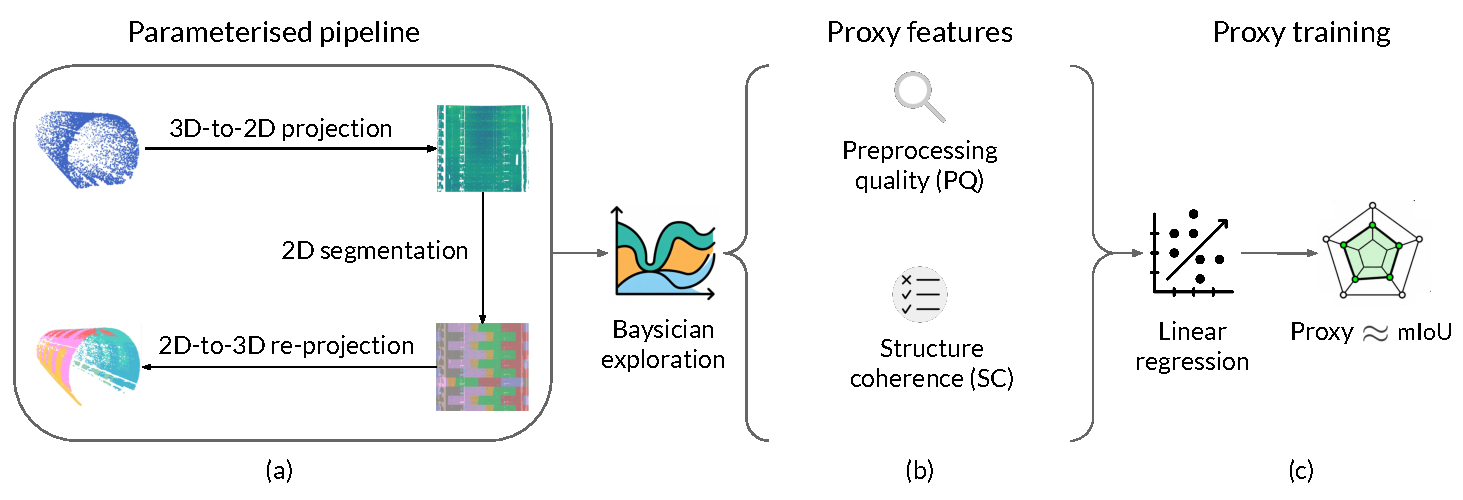
\includegraphics[width=\textwidth]{figs/intrinsics.pdf}
\caption{Development and use of the accuracy proxy. Parameter variations generate segmentation outputs with different accuracies. PQ and SC metrics from each run are paired with GT mIoU to train the proxy. Once fitted, the proxy estimates accuracy on new runs using metrics available without GT. The score is an estimate of segmentation accuracy, not a guarantee of correctness.}
\label{fig:intrinsic_proxy_scoring}
\end{figure*}


\subsection{Task definition}
\label{sec:problem-def}

Given a raw point cloud of a tunnel section, the task is to assign each point either the background label or the label of one lining block. Three block \emph{types} occur in a ring: key (K), adjacent (B), and standard (A). The label set distinguishes the individual blocks within a ring: K, B1, B2, and A1--A3 for staggered and continuous rings (six blocks), and K, B1, B2, and A1--A4 for complex rings (seven blocks), plus background in every family. Seg2Tunnel, the benchmark dataset we use, groups linings into three families (staggered, continuous, and complex). These families differ in ring geometry and acquisition conditions and, most critically for our task, in the key-block (K) layout: ring-to-ring repeating, fixed ring-wise order, and no repeating pattern (Fig.~\ref{fig:task}). 

Given an input point cloud, Proxy4Tun estimates segmentation quality using a learned proxy score computed from PQ/SC metrics. During self-refinement, it evaluates candidate configurations within a predefined parameter space and attempt budget; the proxy score then decides whether to accept the current segmentation, continue refining, or flag the result.

\begin{figure*}[t]
\centering
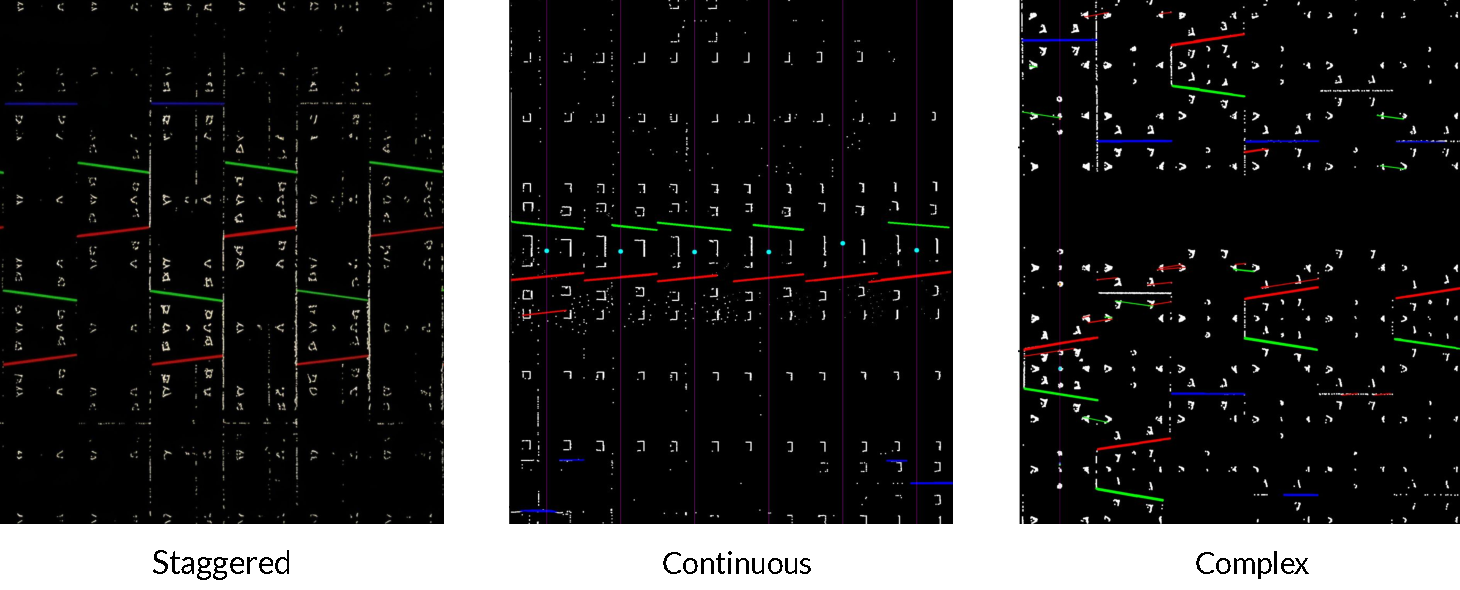
\includegraphics[width=0.8\textwidth]{figs/task.pdf}
\caption{Tunnel-lining block \emph{types} (K, B, A). Evaluation labels distinguish the individual blocks: K, B1, B2, and A1--A3 (six lining classes) or A1--A4 (seven), plus background. mIoU averages over the labels that appear, including background.} 
\label{fig:task}
\end{figure*}




\subsection{Framework overview}
\label{sec:method}

The framework links a parameterised expert-designed segmetation pipeline, a development-time procedure for learning the mIoU proxy, and a deployment-time self-refinement loop that compares candidates using the learnt proxy (Fig.~\ref{fig:intrinsic_proxy_scoring}). Throughout, the pipeline algorithms are fixed and only their parameters vary. 


\subsubsection{Segmentation pipeline}
\label{sec:pipeline}

The pipeline is adapted from SAM4Tun~\cite{ye2025sam4tun} and parameterised for the three Seg2Tunnel lining families~\cite{lin2024seg2tunnel}. Figure~\ref{fig:pipeline} illustrates the processing stages.

\begin{figure*}[t]
\centering
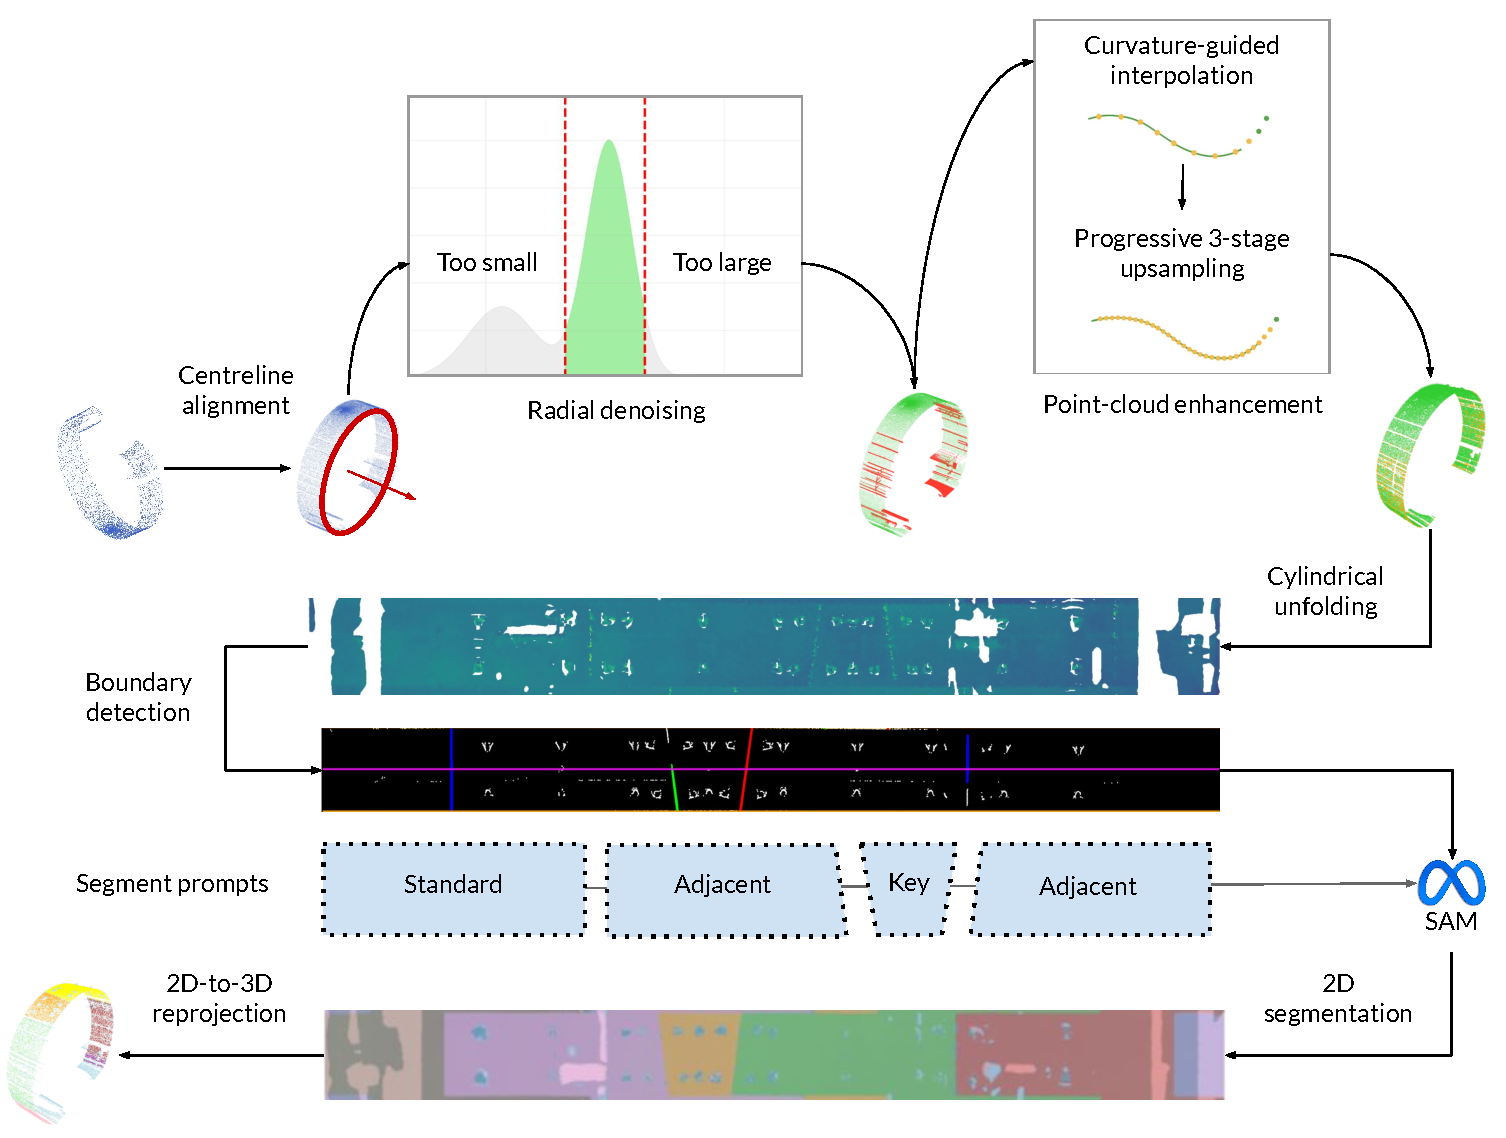
\includegraphics[width=0.98\textwidth]{figs/pipeline.pdf}
\caption{Segmentation pipeline adapted from SAM4Tun. Geometric alignment, filtering, and enhancement produce a depth representation for boundary detection and template-based SAM prompting. The resulting masks are reprojected onto the point cloud. Intermediate outputs provide PQ and SC metrics. The stage algorithms remain fixed; exploration and self-refinement adjust their parameters.}
\label{fig:pipeline}
\end{figure*}

\begin{enumerate}
\item \textbf{Unfolding.}
RANSAC-based cross-sectional ellipse fitting and centreline estimation establish a cylindrical coordinate system~\cite{fischler1981ransac}. The lining surface is represented panoramically, with depth describing radial distance from the centreline. Coordinate orientation is fixed so that block positions retain the same meaning across runs.

\item \textbf{Denoising.}
Radial masks and grid-based point-density filtering remove points inconsistent with the expected lining surface. The filtering follows the density-based principle underlying DBSCAN~\cite{ester1996dbscan}. Its settings affect both unwanted-point removal and the amount of lining data retained.

\item \textbf{Enhancement.}
Curvature-guided interpolation and progressive upsampling improve the completeness of the depth representation before detection, while preserving joint boundaries.

\item \textbf{Boundary detection.}
Orientation-specific Hough transforms identify candidate ring and block boundaries~\cite{duda1972hough}. These detections are organised according to the expected family layout.

\item \textbf{Segmentation and reprojection.}
The detected layout defines template-based prompts for SAM~\cite{kirillov2023sam}. The resulting image masks are mapped back to the point cloud to obtain three-dimensional block labels.
\end{enumerate}

This adapted pipeline is used for both calibration and self-refinement. Only its parameter settings vary within prescribed family-specific bounds; the stage algorithms and SAM model weights remain fixed (Appendix~\ref{app:anchor-parameter}). Each run produces a segmentation output and PQ/SC metrics for proxy-based quality assessment.

\subsubsection{Generating calibration examples}
\label{sec:bo-experience}
Calibration requires examples linking PQ/SC metrics to segmentation accuracy across successful and degraded parameter settings. Each lining family has an expert reference configuration, tuned by the pipeline developers on one labelled development subset before this study. We vary its parameters within prescribed bounds and reuse the same subset's annotations to calculate GT mIoU for each run, producing 120 calibration examples across three development subsets. The family references also provide the starting configurations for self-refinement.

Two sampling stages balance coverage and informativeness within each lining family. First, scrambled Sobol sampling provides 32 valid trials spread across the prescribed parameter ranges~\cite{joe2008constructing}, allowing exploration of both successful and degraded settings. Second, Bayesian exploration adds eight valid trials where a Gaussian-process (GP) model of GT mIoU has the highest predictive uncertainty~\cite{gramacy2009adaptive,gramacy2020surrogates}. We target uncertainty rather than maximise accuracy because the proxy must estimate and rank segmentation quality across a range of accuracies, rather than identify a single optimum (Appendix~\ref{app:bo-config}). Each valid run records its parameter configuration, PQ/SC metrics, and GT mIoU. Algorithm~\ref{alg:bo_exploration} and Figure~\ref{fig:b-p} summarise the procedure; Appendix~\ref{app:search-bounds} lists the parameter bounds.

\begin{figure*}[t]
\centering
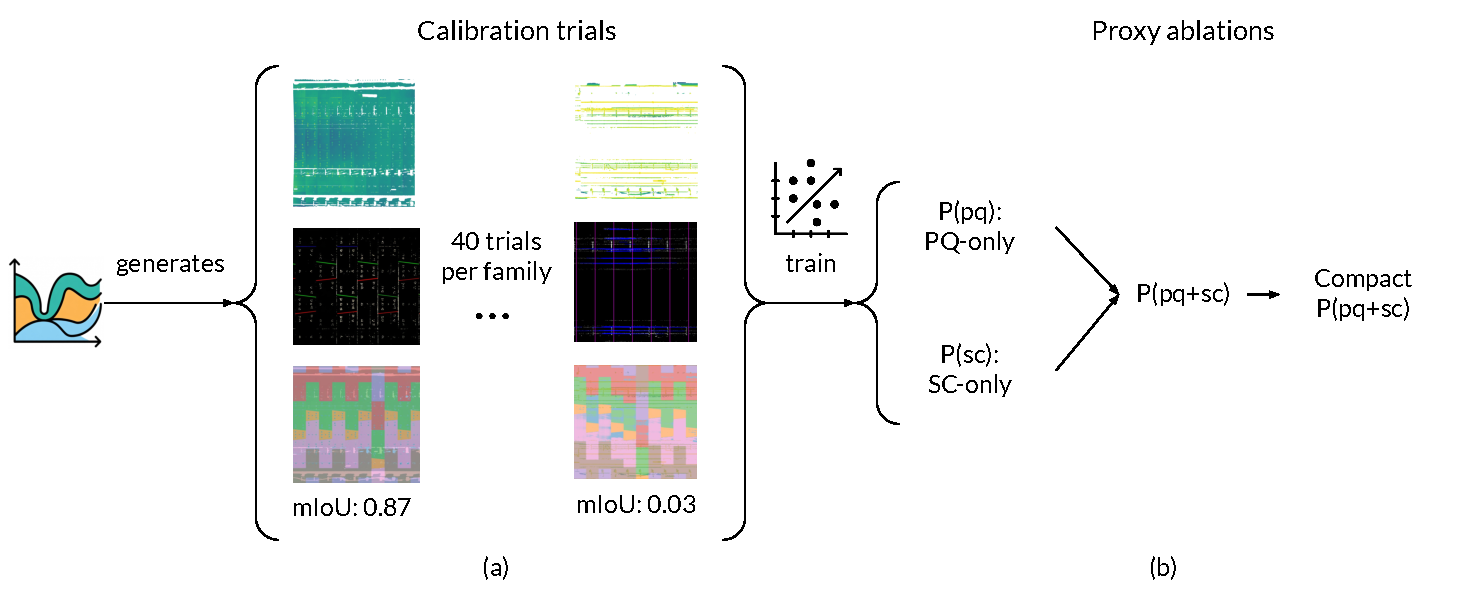
\includegraphics[width=\textwidth]{figs/b-p.pdf}
\caption{Calibration-example generation and feature comparison.
(a) Each lining family contributes 32 valid scrambled-Sobol trials
and eight valid Bayesian exploration trials selected by GP
uncertainty. All trials reuse the same development-subset annotations.
(b) The resulting metrics and GT mIoU values support comparison
of PQ-only, SC-only, combined, and compact combined feature sets
for the accuracy proxy.}
\label{fig:b-p}
\end{figure*}

\begin{algorithm}[ht]
\caption{Generating calibration examples through space-filling
sampling and Bayesian exploration}
\label{alg:bo_exploration}
\begin{algorithmic}[1]
\Require Development subset $D_f$ with GT annotations $Y_f$
\Require Reference configuration $P_f^{\mathrm{ref}}$; expected ring count $N_{\mathrm{exp}}=10$
\Require Parameter bounds $\Theta_f$;
         valid-trial budgets $N_0=32$, $N_1=8$;
         candidate-pool size $M=2048$
\Ensure Calibration records $\mathcal{T}_f$
\State $\mathcal{T}_f\gets\emptyset$;
       $n_0\gets0$; $n_1\gets0$
\State Initialise a scrambled-Sobol sequence
\Statex \textit{Phase 1: broad initial coverage}
\While{$n_0<N_0$}
    \State Draw the next Sobol point and map it to
           permitted parameter values $\theta\in\Theta_f$
    \State $P\gets\operatorname{Apply}
           (P_f^{\mathrm{ref}},\theta)$
    \State $R\gets\operatorname{Pipeline}(D_f,P)$
    \If{$R$ is valid and required metrics are available}
        \State $\mathbf{x}\gets\operatorname{Features}(R,N_{\mathrm{exp}})$
        \State $y\gets\operatorname{mIoU}(R,Y_f)$
        \State Append $(\theta,\mathbf{x},y)$
               to $\mathcal{T}_f$
        \State $n_0\gets n_0+1$
    \Else
        \State Log the failed or incomplete trial
    \EndIf
\EndWhile
\Statex \textit{Phase 2: Bayesian exploration}
\State Fit GP to the $(\theta,y)$ pairs in $\mathcal{T}_f$
\While{$n_1<N_1$}
    \State Draw $M$ random candidate settings
           $\mathcal{P}_t$ within $\Theta_f$
    \State $\theta\gets
           \arg\max_{\vartheta\in\mathcal{P}_t}
           \sigma_t(\vartheta)$
    \State $P\gets\operatorname{Apply}
           (P_f^{\mathrm{ref}},\theta)$
    \State $R\gets\operatorname{Pipeline}(D_f,P)$
    \If{$R$ is valid and required metrics are available}
        \State $\mathbf{x}\gets\operatorname{Features}(R,N_{\mathrm{exp}})$
        \State $y\gets\operatorname{mIoU}(R,Y_f)$
        \State Append $(\theta,\mathbf{x},y)$
               to $\mathcal{T}_f$
        \State Update GP using the expanded $\mathcal{T}_f$
        \State $n_1\gets n_1+1$
    \Else
        \State Log the failed or incomplete trial
    \EndIf
\EndWhile
\State \Return $\mathcal{T}_f$
\end{algorithmic}
\end{algorithm}

\subsubsection{PQ and SC metrics}
\label{sec:features}

Metrics form two groups that capture two aspects of pipeline quality: upstream, where the depth representation may be incomplete or misaligned (PQ), and downstream, where the recovered layout may be incoherent even when the input is sound (SC). Table~\ref{tab:candidate-features} lists the ten candidate metrics (four PQ, six SC), whose relationship with segmentation accuracy is assessed during calibration using GT mIoU. SC is particularly relevant to the complex family, where the key block does not repeat from ring to ring while the retained SC features still apply: they count the rings, match block boundaries to detected joints, and measure how much of the point cloud receives a block label. However, high structural coherence does not guarantee correctness: because joint detections also drive SAM prompting, detected joints and predicted boundaries may agree while sharing the same underlying error. Their agreement is evidence, not proof, of correctness.

\begin{table*}[t]
\caption{Candidate metrics for the mIoU accuracy proxy (four PQ, six SC). Pixel quantities refer to the 5\,mm depth-image grid. The four retained by the frozen proxy are marked $\star$. Stages: 1---unfolding; 2---denoising; 3---enhancement; 4---joint detection; 5---SAM segmentation. Combined indices indicate metrics using outputs from both stages.}
\label{tab:candidate-features}
\centering
\small
\setlength{\tabcolsep}{3pt}
\begin{tabular}{p{0.05\textwidth} p{0.27\textwidth} p{0.45\textwidth} p{0.16\textwidth}}
\toprule
Group & Measurement & Meaning & Stage \\
\midrule
PQ & Unfolding fit residual & Centreline fit error & 1 \\
 & Orientation agreement & Agreement between the inferred axis and the recorded travel direction & 1 \\
 & Point retention & Fraction of input points kept after denoising & 2 \\
 & Missing-depth rate $\star$ & Fraction of all depth-image pixels without depth after enhancement & 3 \\
SC & Ring-count residual $\star$ & $|N_{\mathrm{det}}-N_{\mathrm{exp}}|$ in rings against the acquisition record ($N_{\mathrm{exp}}=10$) & 4 \\
 & Edge support & Fraction of label-boundary pixels within 25\,px of a depth edge & 3+5 \\
 & Correspondence score $\star$ & F1 at 15\,px between rasterised joint lines and block--block boundaries (empty detection $\Rightarrow 0$) & 4+5 \\
 & Line--boundary distance & Symmetric mean distance (capped at 200\,px) between joints and boundaries & 4+5 \\
 & Fill rate $\star$ & Fraction of all input points assigned a non-background label & 5 \\
 & Phase incoherence & Inconsistency of label ordering across rings & 5 \\
\bottomrule
\end{tabular}
\end{table*}

\subsubsection{Learning the accuracy proxy}
\label{sec:ridge-proxy}

The proxy maps PQ and SC metrics to an estimated mIoU. We fit ridge-regression proxies using candidate feature sets and compare them through LOFO validation to select a compact model. Regularisation stabilises estimation under correlated predictors~\cite{hoerl1970ridge,pedregosa2011sklearn}, while the linear form \hl{allows the estimator to be inspected by the LLMs}. The coefficients represent fitted associations, not causal prescriptions for parameter changes. We choose this model form for interpretable feedback and do not claim predictive superiority over nonlinear alternatives.

For a feature vector $\mathbf{x}\in\mathbb{R}^{d}$, the prediction is
\begin{equation}
\hat{y}(\mathbf{x})
=
b+\sum_{j=1}^{d}
w_j\frac{x_j-\mu_j}{s_j},
\label{eq:ridge-proxy}
\end{equation}
where $d$ is the number of features, $\mu_j$ and $s_j$ are the training-set mean and standard deviation of feature $j$, $w_j$ is its fitted coefficient, and $b$ is the intercept. Coefficients are fitted by minimising squared prediction error with an $\ell_2$ penalty of strength $\alpha$.

We compare four prespecified feature sets: PQ-only $P(q)$, SC-only $P(c)$, combined $P(q{+}c)$, and compact combined models (Table~\ref{tab:proxy-ablation}). Each LOFO fold trains on two families and evaluates on the third, with feature scaling, penalty selection, and coefficient fitting restricted to the training families. Predictions across the three held-out folds are pooled to calculate Spearman $\rho$ and MAE over all 120 calibration runs; per-family $\rho$ is also reported. The feature set with the highest pooled LOFO $\rho$ is selected, and the final model is fitted on all 120 calibration runs and frozen. Algorithm~\ref{alg:proxy} summarises model development and deployment scoring.

\begin{table}[ht]
\caption{Prespecified proxy feature sets compared under LOFO validation.}
\label{tab:proxy-ablation}
\centering
\begin{tabular}{p{0.38\columnwidth} p{0.52\columnwidth}}
\toprule
Model & Definition \\
\midrule
$P(q)$ & Four PQ features \\
$P(c)$ & Six SC features \\
$P(q{+}c)$ & All ten candidate features \\
Compact $P(q{+}c)$ & Four prespecified features: one PQ and three SC \\
\bottomrule
\end{tabular}
\end{table}

\begin{algorithm}[ht]
\caption{Proxy calibration and deployment scoring}
\label{alg:proxy}
\begin{algorithmic}[1]
\Require Calibration records $\mathcal{T}=\bigcup_f\mathcal{T}_f$; prespecified candidate feature sets; fixed feature-extraction conventions
\Ensure Frozen proxy $g$ and deployment score $\hat{y}$
\For{each candidate feature set $V$}
    \For{each held-out family $f$}
        \State Use the other two families as training data
        \State Fit feature scaling and select $\alpha$ using only the training data
        \State Fit ridge regression and predict the held-out family's mIoU
        \State Clip predictions to $[0,1]$
    \EndFor
    \State Pool predictions across the three folds
    \State Record pooled Spearman $\rho$ and MAE, and per-family $\rho$
\EndFor
\State Select the feature set with the highest pooled LOFO $\rho$
\State Fit final scaling and ridge regression on all 120 calibration records
\State Freeze feature definitions, order, scaler, coefficients, and intercept as $g$
\Statex
\State Receive a completed run $r$ and its expected ring count $N_{\mathrm{exp}}$
\State $\mathbf{x}\gets\operatorname{Features}(r,N_{\mathrm{exp}})$ in the frozen feature order
\State $\hat{y}\gets\min(1,\max(0,g(\mathbf{x})))$
\State \Return $\hat{y}$
\end{algorithmic}
\end{algorithm}


\subsection{Proxy-guided parameter self-refinement}
\label{sec:agent-design}

The proxy estimates accuracy but does not decide which parameters to change. Each LLM agent (GPT-5.6, Fable-5.1, or Gemini-3.8), evaluated separately, proposes a parameter change (Fig.~\ref{fig:agent}). It receives the family reference, the current run's intermediate outputs and PQ/SC metrics, the proxy score, and short engineering notes linking observable symptoms to likely adjustments (Appendices~\ref{app:ontology} and~\ref{app:prompt}). It returns one bounded parameter update with a brief rationale.

\paragraph{Shared protocol.}
Each of the 27 subsets starts from its expert family reference and receives three proposal attempts per arm, without proxy-based admission screening or early stopping. All arms share the parameter bounds, attempt budget, and retention rule. \hl{Each attempt modifies only the parameters it calls, and the shared retention rule decides whether that candidate replaces the current output. } Invalid or failed proposals consume an attempt, so equal budgets do not necessarily imply equal numbers of pipeline executions or equal runtime.

\paragraph{Adaptive-random control.}
The control samples the number of parameters to change from an empirical distribution obtained from an earlier LLM pilot, then randomly selects parameters and values within the allowed bounds (Appendix~\ref{app:random-search}). This distribution is frozen before the experiment. Random updates are applied to the retained configuration without using intermediate metrics or images to guide sampling. In all arms, however, unfolding parameters are eligible for modification only when the starting centreline residual exceeds $10\,\mathrm{cm}$. The comparison evaluates proposal strategies under common constraints; it does not isolate LLM reasoning from differences in proposal size or parameter choice.

\paragraph{Execution and feedback.}
Each proposal is checked against the allowed parameter names, types, and ranges. Valid proposals are executed through the pipeline, and the resulting PQ/SC metrics are scored by the frozen proxy. The proposed update, score, and outcome are recorded. For the LLM arms, this record provides feedback for subsequent attempts, together with the retained configuration and its outputs as the current state.

\paragraph{Retention.}
A candidate replaces the currently retained output only if its proxy score, clipped to $[0,1]$, exceeds the retained score by more than the predefined margin of $0.01$; otherwise, the retained output remains unchanged. The same rule applies to all arms. Algorithm~\ref{alg:reflective_adaptation} summarises the loop.

\begin{figure*}[t]
\centering
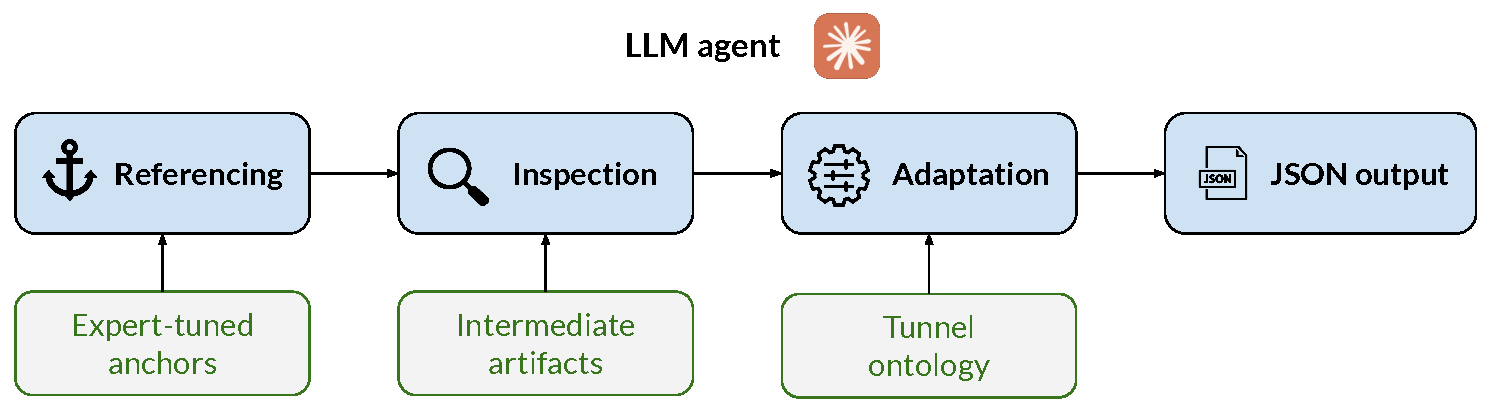
\includegraphics[width=0.8\textwidth]{figs/agent.pdf}
\caption{LLM-guided parameter proposals. The agent compares the current run with engineering references, inspects intermediate outputs and PQ/SC metrics, and returns a bounded parameter update with a rationale. After execution, the frozen proxy scores the candidate. Candidate retention depends only on the proxy score.}
\label{fig:agent}
\end{figure*}

\begin{algorithm}[ht]
\caption{Proxy-guided parameter self-refinement}
\label{alg:reflective_adaptation}
\begin{algorithmic}[1]
\Require Input point-cloud subset; expert reference configuration; frozen proxy; parameter bounds
\Ensure Retained configuration, segmentation output, and proxy score
\State Run the expert reference and retain its configuration and output
\State Compute its proxy score, clipped to $[0,1]$
\For{attempt $=1,2,3$}
    \State Propose one update using the LLM or adaptive-random strategy
    \State Validate parameter names, types, bounds, and eligibility
    \If{the update is invalid}
        \State Record the failure and continue to the next attempt
    \EndIf
    \State Execute the candidate configuration
    \If{execution fails}
        \State Record the failure and continue to the next attempt
    \EndIf
    \State Compute PQ/SC metrics and the candidate proxy score, clipped to $[0,1]$
    \If{candidate score $>$ retained score $+\,0.01$}
        \State Retain the candidate configuration, output, and score
    \EndIf
    \State Record the update, metrics, score, and retention outcome
    \State Make the record and retained state available to the next LLM proposal
\EndFor
\State \Return retained configuration, segmentation output, and proxy score
\end{algorithmic}
\end{algorithm}


\subsection{Experimental setup}
\label{sec:exp-setup}

\subsubsection{Dataset and reference configurations}
\label{sec:dataset}
We use 30 ten-ring subsets from five parent tunnels in Seg2Tunnel, covering staggered, continuous, and complex lining families~\cite{lin2024seg2tunnel}. One labelled development subset per family supplies 40 calibration runs; the remaining 27 subsets are held out for evaluation (Table~\ref{tab:dataset}). A single proxy is fitted to calibration runs pooled across all three lining families and evaluated on the 27 held-out subsets. Where we report bootstrap confidence intervals, we account for shared geometry and acquisition conditions by resampling at the parent-tunnel level unless stated otherwise (Section~\ref{sec:sensitivity}).


Each expert family reference was tuned by the pipeline developers on the corresponding development subset, with its annotations available, and established before this study. It provides the basis for calibration and the unchanged starting configuration for held-out evaluation and self-refinement. Development annotations support reference assessment and supply calibration targets; held-out annotations are used only for retrospective evaluation. Appendices~\ref{app:anchor-parameter} and~\ref{app:search-bounds} list the reference configurations and exploration bounds, respectively.

\hl{One additional subset from the STSD dataset is included as an external control. It has a complex lining layout and no STSD-specific expert reference; it is analysed separately from the Seg2Tunnel panel and is not pooled with the main results.}

\begin{table*}[t]
\caption{Development and held-out subsets. One labelled development subset per family supplies the calibration trials; nine other subsets per family form the held-out evaluation data.}
\label{tab:dataset}
\centering
\begin{tabular}{p{0.22\textwidth} p{0.24\textwidth} p{0.22\textwidth} p{0.22\textwidth}}
\toprule
Property & Staggered (T1, T2) & Continuous (T3) & Complex (T4, T5) \\
\midrule
Inner diameter & 5.5\,m & 5.9\,m & 7.5\,m \\
Ring length & 1.2\,m & 1.2\,m & 1.8\,m \\
Blocks per ring & 6 & 6 & 7 \\
Key-block layout & Ring-to-ring repeating pattern & Fixed ring-wise order & No repeating pattern \\
Scanning & Single-station & Multi-station & Single-station, offset \\
Development subset & 2-1 & 3-1 & 5-1 \\
Calibration runs & 40 & 40 & 40 \\
Held-out subsets & 1-1 to 1-5; 2-2 to 2-5 & 3-2 to 3-10 & 4-1-to 4-5; 5-2 to 5-5 \\
\bottomrule
\end{tabular}
\end{table*}


\subsubsection{Feature and model comparisons}
\label{sec:comparators}

We use the 120 calibration runs for two checks. First, we compare how well each feature set fits the training data and predicts accuracy for a family excluded from fitting (LOFO; Table~\ref{tab:proxy-ablation}). Second, we shuffle GT mIoU values within each family and repeat LOFO fitting 20 times. This breaks run-level relationships while preserving family differences, testing whether the metrics predict accuracy beyond family identity. The final frozen proxy is then evaluated on held-out data.

\subsubsection{Paired degradation test}
\label{sec:stress-test}

For each of the 27 held-out subsets, we run the family reference and a deliberately degraded configuration (Appendix~\ref{app:degradation}). Both configurations process the same input point cloud, avoiding differences between scans. GT mIoU is calculated afterwards to confirm degradation. We evaluate how accurately the frozen proxy estimates mIoU and whether it ranks each reference output above its degraded counterpart. This tests ranking under controlled degradation rather than reliability on naturally occurring failures.

\subsubsection{Self-refinement against family-specific references}
\label{sec:poc-protocol}

We compare four proposal arms on all 27 held-out subsets: GPT-5.6, Fable-5.1, Gemini-3.8, and adaptive-random search. Each starts from the same expert family reference and receives three attempts, sharing the frozen proxy, parameter bounds, and retention rule, without admission screening or early stopping (Algorithm~\ref{alg:reflective_adaptation}; Fig.~\ref{fig:verification}). Table~\ref{tab:poc-config} lists the study configuration.

\begin{figure*}[t]
\centering
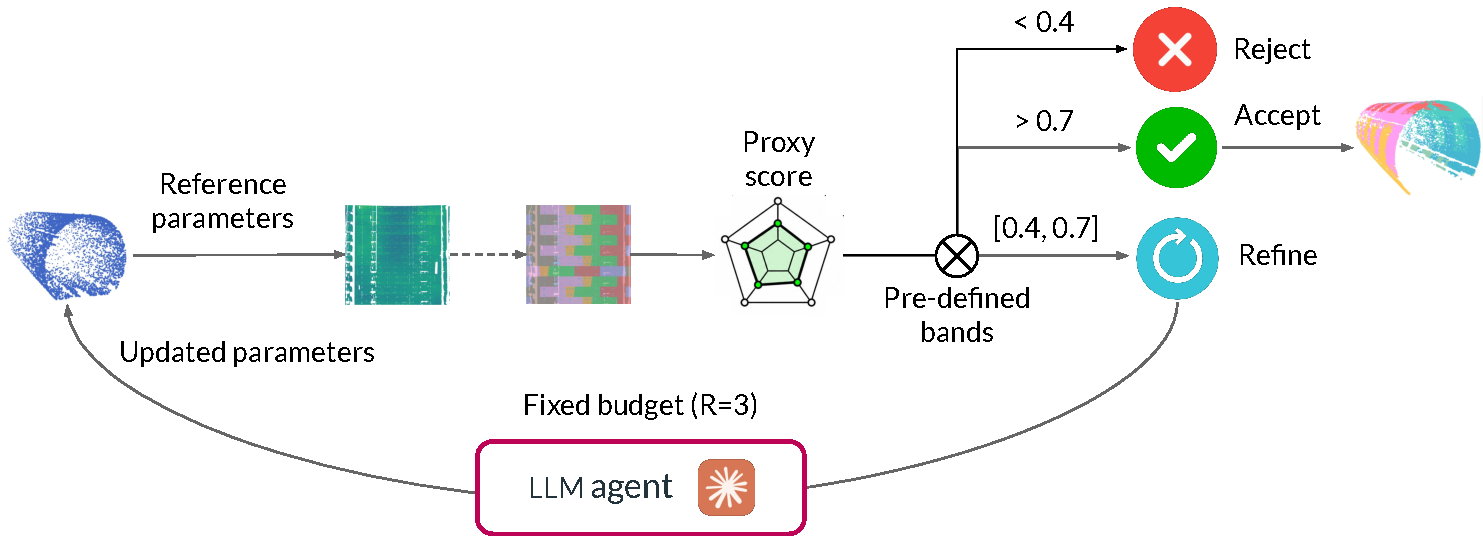
\includegraphics[width=0.9\textwidth]{figs/verification.pdf}
\caption{Self-refinement protocol shared by all arms. Each of the 27 expert-reference starts receives three proposal attempts per arm. Invalid or failed attempts consume budget and leave the retained configuration unchanged. A candidate is retained only if its proxy score exceeds the current retained score by more than $0.01$.}
\label{fig:verification}
\end{figure*}

Each LLM agent receives the reference, bounds, engineering notes, PQ/SC metrics, proxy scores, and rendered depth maps, detected lines, prompt points, and segmentation images. One session per subset and LLM arm is resumed across attempts to preserve proposal history and feedback, with no access to GT, evaluation directories, or other arms. All 324 proposals and outcomes are logged ($27$ subsets $\times 4$ arms $\times 3$ attempts), comprising 243 LLM proposals and 81 adaptive-random proposals, and pipeline runs use a single NVIDIA RTX~5060 GPU.

\begin{table}[ht]
\caption{Self-refinement study configuration.}
\label{tab:poc-config}
\centering
\begin{tabular}{p{0.35\columnwidth} p{0.55\columnwidth}}
\toprule
Setting & Value \\
\midrule
Proposal arms & GPT-5.6; Fable-5.1; Gemini-3.8; adaptive-random search \\
LLM identifiers & \texttt{gpt-5.6-sol-medium}; \texttt{claude-fable-5-1-thinking-high}; Gemini~3.8 as the active agent model \\
Interface & One coding-agent session per subset and LLM arm, resumed across attempts \\
Starting configuration & Expert family reference \\
Evaluation cases & All 27 held-out subsets \\
Context (LLM arms) & Engineering notes, pipeline outputs, PQ/SC metrics, and proxy scores; no GT \\
Budget & Three proposal attempts per subset and arm \\
Early stopping & None \\
Output & One JSON parameter update per attempt, with a rationale for LLM arms \\
Failure handling & Invalid or failed attempts consume budget; retained output remains unchanged \\
Retention & Candidate proxy score exceeds the current retained score by more than $0.01$ \\
\bottomrule
\end{tabular}
\end{table}


\subsubsection{Evaluation metrics}
\label{sec:metrics}

Segmentation accuracy is evaluated retrospectively against GT using point-wise semantic mIoU:
\begin{equation}
\operatorname{IoU}_c
=
\frac{\operatorname{TP}_c}
{\operatorname{TP}_c+\operatorname{FP}_c+\operatorname{FN}_c},
\qquad
\operatorname{mIoU}
=
\frac{1}{C}\sum_{c=1}^{C}\operatorname{IoU}_c,
\end{equation}
where $\operatorname{TP}_c$, $\operatorname{FP}_c$, and $\operatorname{FN}_c$ are the true-positive, false-positive, and false-negative point counts for label $c$, and $C$ is the number of labels included in the average for that subset (labels present in either GT or prediction, including background). In this study, $C=7$ for staggered and continuous subsets and $C=8$ for complex subsets.

Proxy performance is measured by Spearman $\rho$ for agreement with GT accuracy rankings and mean absolute error (MAE), defined as the mean absolute difference between predicted and GT mIoU. In the paired degradation test, we also report the proportion of pairs in which the reference receives a higher proxy score than its degraded counterpart; ties count as failures.

For self-refinement, we report proxy scores and GT mIoU before and after refinement. For each proposal strategy, we subtract each subset's initial GT mIoU from its final GT mIoU and average these changes across the 27 subsets. \hl{Averaging across the 27 subsets gives equal weight to each lining family, since each contributes nine subsets.} Proposal quality is assessed relative to the expert-reference start: a proposal is classified as harmful if its GT mIoU is more than $0.05$ lower than the starting value.

\subsubsection{Statistical uncertainty}
\label{sec:sensitivity}

\hl{The reported mean gain is the unweighted mean of the 27 subset changes. Its interval is a different quantity. Each parent tunnel is first reduced to its own mean gain. A resample draws those five tunnel means with replacement and averages them with equal weight. The 95\% interval is the 2.5 and 97.5 percentiles of that average over 100{,}000 resamples. Equal family counts do not make this the 27-subset mean: the five tunnels contribute 5, 4, 9, 5, and 4 subsets. The error bars in Fig.}~\ref{fig:assume_random_comparison}\hl{ use this same tunnel-mean interval.} Intervals are interpreted cautiously because only five parent tunnels are available.

\subsubsection{Sensitivity to LLM choice}
\label{sec:llm-sensitivity}

We assess how self-refinement outcomes depend on the proposing LLM by comparing GPT-5.6, Fable-5.1, and Gemini-3.8 under identical starting configurations, parameter bounds, attempt budgets, and proxy-based retention. We compare final mIoU, changes from the expert-reference baseline, harmful-proposal rates, and the numbers of improved, unchanged, and worsened subsets. These comparisons examine whether the observed benefits are consistent across the three models or concentrated in one. Each model is evaluated once per subset, so the analysis describes differences between models rather than variability across repeated sessions.


\section{Results}\label{sec:results}
% ══════════════════════════════════════════════════════════════════════════

The results follow the three questions of Section~\ref{sec:exp-setup}: whether PQ and SC carry accuracy information that transfers across families, whether the frozen proxy separates references from degradations on \hl{held-out tunnel sections}, and whether it can guide refinement of already-strong references. A residual error analysis then examines failure modes that the four-feature proxy does not reliably detect.

\subsection{Proxy calibration and feature ablation}
\label{sec:main-results}
\label{sec:proxy-ablation-results}

\hl{The selected proxy contains three SC metrics (correspondence F1@15, segmentation fill rate, and assumed-line count) and one PQ metric (depth-map invalid-pixel fraction). Assumed-line count is the number of fallback joint lines marked \texttt{assume} by the detector. With training-standardised inputs, its fitted equation is}
\begin{equation}
\begin{aligned}
\hat{y}={}&\colorbox{yellow}{$\displaystyle 0.358867+0.088443z_{\mathrm{corr}}+0.105800z_{\mathrm{fill}}$}\\
&\colorbox{yellow}{$\displaystyle -0.021558z_{\mathrm{assume}}-0.033997z_{\mathrm{nan}}$}.
\end{aligned}
\label{eq:four-proxy}
\end{equation}
\hl{Each $z$ denotes the corresponding metric standardised using the calibration-set mean and standard deviation. RidgeCV selects $\alpha=5.623413$. Greater correspondence and coverage increase the estimate, while assumed lines and invalid depth decrease it, holding other inputs constant. These are conditional associations in a correlated linear model, not causal effects.}

\begin{figure*}[t]
\centering
\begin{hlbox}
\centering
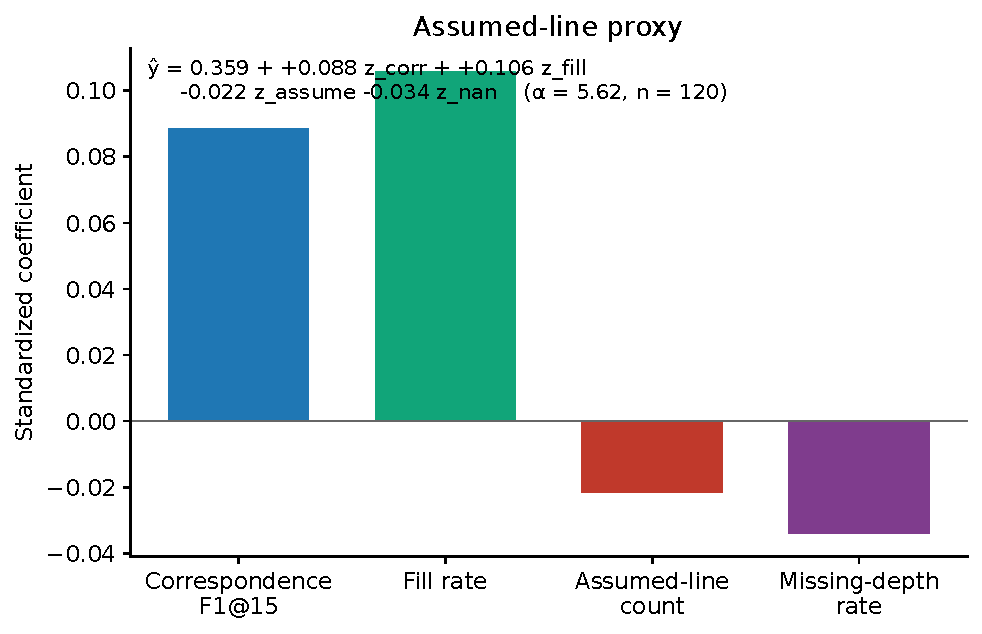
\includegraphics[width=0.92\textwidth]{figs/assume_proxy_formula.pdf}
\end{hlbox}
\caption{\hl{The assumed-line proxy. The compact model combines correspondence, fill, assumed-line, and invalid-depth evidence on a shared standardised scale.}}
\label{fig:assume_proxy_formula}
\end{figure*}

\begin{table*}[t]
\caption{\hl{Proxy calibration and LOFO transfer for the compact model.}}\label{tab:proxy-calibration}
\begin{tabular*}{\textwidth}{@{\extracolsep{\fill}} l c c @{}}
\toprule
Setting & MAE & Spearman \\
\midrule
\rowcolor{yellow!25}Training fit ($n = 120$) & 0.108 & 0.863 \\
\rowcolor{yellow!25}Permutation control (20 shuffles, LOFO) & -- & $-0.122\pm0.093$ \\
\rowcolor{yellow!25}Leave-one-family-out & 0.145 & 0.754 \\
\bottomrule
\end{tabular*}
\end{table*}

\hl{Table~\ref{tab:proxy-calibration} reports the fit.} \hl{Correlation decreases from $0.863$ in training to $0.754$ under LOFO.} \hl{The within-family permutation control gives} $\hl{\rho=-0.122\pm0.093}$\hl{. Useful ranking therefore remains when a family is excluded and is not explained by family identity alone.}

\begin{table*}[t]
\caption{\hl{Proxy feature-set comparison under LOFO. Family columns give Spearman correlation on each held-out family.}}\label{tab:ablation-results}
\begin{tabular*}{\textwidth}{@{\extracolsep{\fill}} l c cccc c @{}}
\toprule
Condition & \#Features & Pooled $\rho$ & Staggered & Continuous & Complex & LOFO MAE \\
\midrule
\rowcolor{yellow!25}$P(q)$ (PQ only) & 4 & 0.615 & 0.595 & 0.551 & 0.466 & 0.166 \\
\rowcolor{yellow!25}$P(c)$ (SC only) & 6 & 0.715 & 0.834 & 0.358 & 0.866 & 0.155 \\
\rowcolor{yellow!25}$P(q{+}c)$ (combined) & 10 & 0.744 & 0.869 & 0.263 & \textbf{0.936} & 0.148 \\
\rowcolor{yellow!25}Compact $P(q{+}c)$ (deployed) & \textbf{4} & \textbf{0.754} & \textbf{0.883} & \textbf{0.479} & 0.861 & \textbf{0.145} \\
\bottomrule
\end{tabular*}
\end{table*}

\hl{The compact set gives the strongest pooled transfer and lowest MAE (Table~\ref{tab:ablation-results}). The learning curve rises from $\rho=0.641\pm0.174$ at five runs per family to $0.699\pm0.086$ at ten, $0.723\pm0.062$ at 15, $0.753\pm0.047$ at 20, and $0.750\pm0.032$ at 30, reaching $0.754$ with all 40. Most transfer performance is therefore present by approximately 20 calibration runs per family, with decreasing variability.}

\begin{figure*}[t]
\centering
\begin{hlbox}
\centering
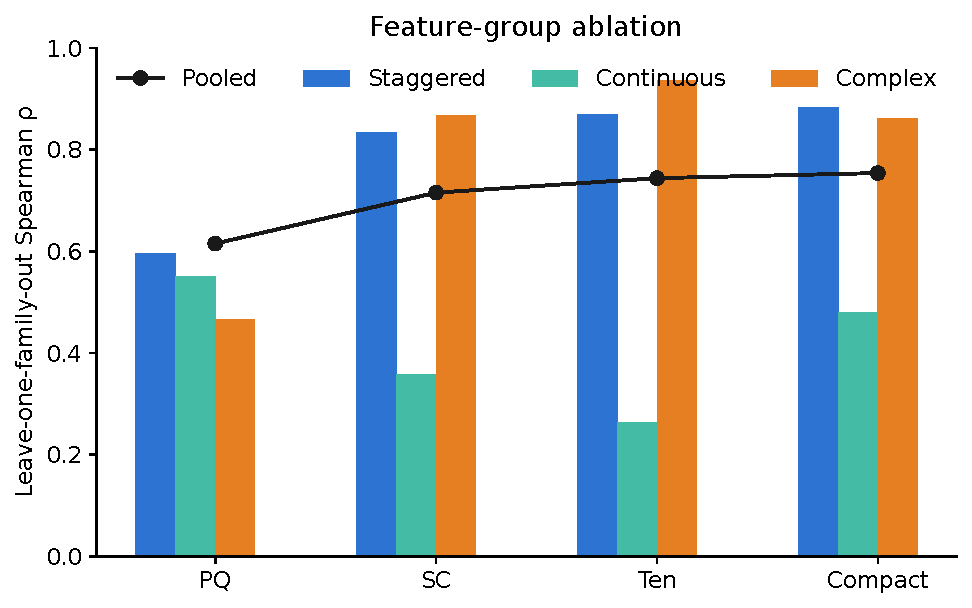
\includegraphics[width=0.92\textwidth]{figs/assume_feature_ablation.pdf}
\end{hlbox}
\caption{\hl{Feature-set transfer, permutation check, and calibration learning curve. Compact PQ+SC gives the highest pooled LOFO rank correlation.}}
\label{fig:assume_feature_ablation}
\end{figure*}

\subsection{\hl{Proxy reliability on constructed and natural outputs}}
\label{sec:holdout}

\hl{On the 54 held-out runs, the frozen proxy reaches Spearman $\rho=0.789$ (95\% CI $[0.711,0.858]$) and MAE $=0.106$. It ranks all 27 reference--degradation pairs correctly. The highest degraded score is $0.179$ and the lowest reference score is $0.412$, so a $0.4$ gate separates the constructed failures with precision and recall both equal to 1.000.}

\begin{figure*}[t]
\centering
\begin{hlbox}
\centering
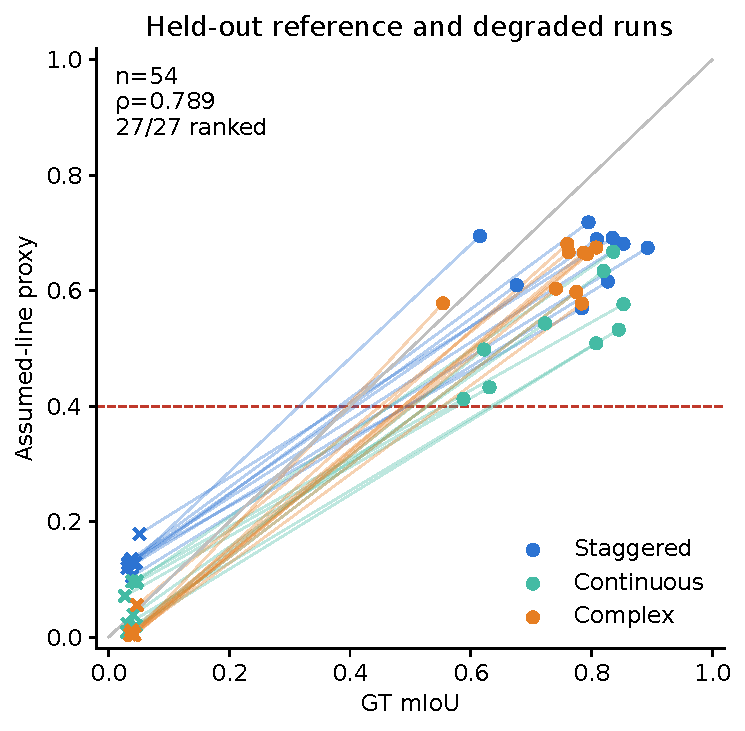
\includegraphics[width=0.92\textwidth]{figs/assume_holdout_ranking.pdf}
\end{hlbox}
\caption{\hl{Held-out proxy reliability. The frozen proxy separates expert references from deliberately degraded runs and correctly orders every paired comparison.}}
\label{fig:assume_holdout_ranking}
\end{figure*}

\hl{The same proxy remains informative on 324 naturally generated proposal outputs: $\rho=0.516$ (95\% CI $[0.400,0.680]$) and MAE $=0.141$. All 18 outputs with GT mIoU below $0.3$ score below $0.4$; the highest score among them is $0.294$. At a proxy threshold of $0.4$, recall is 1.000, 0.958, and 0.839 for GT mIoU below 0.3, 0.4, and 0.5, respectively. Among the 27 expert-reference starts, the operating bands assign one to accept, 26 to refine, and none to flag.}

\begin{figure*}[t]
\centering
\begin{hlbox}
\centering
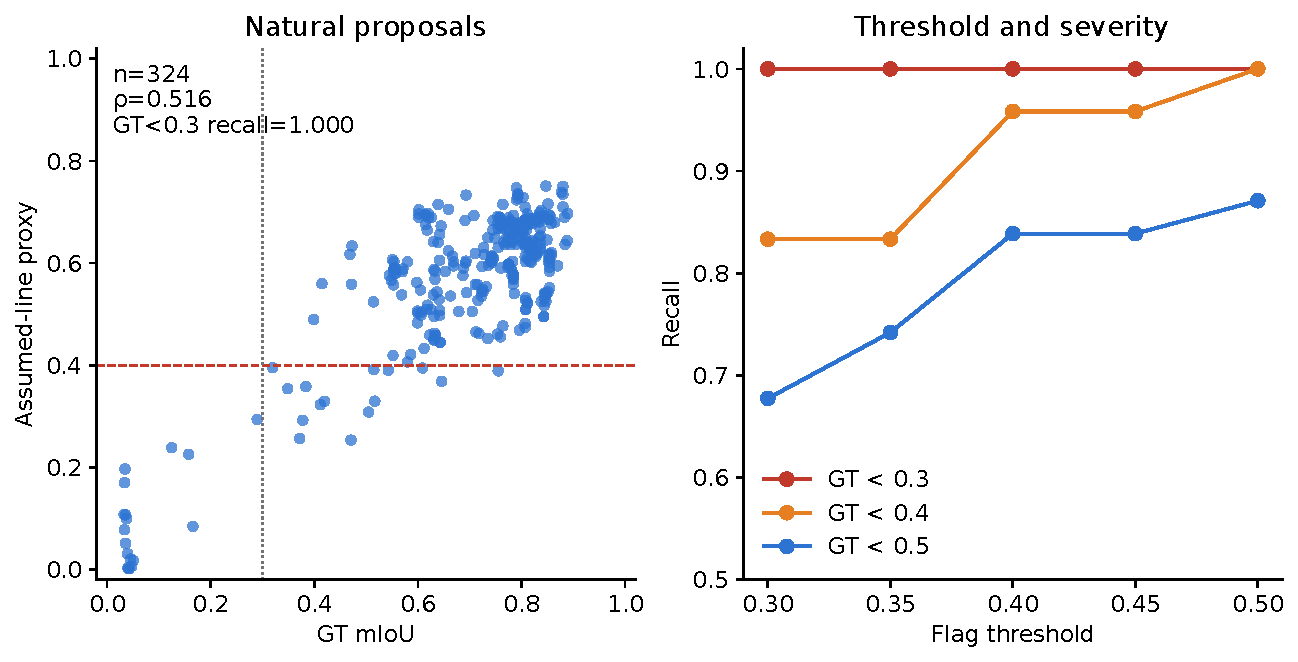
\includegraphics[width=0.92\textwidth]{figs/assume_natural_gate.pdf}
\end{hlbox}
\caption{\hl{Natural-proposal gate evaluation. The proxy is less precise on close natural variants than on constructed degradations, but the $0.4$ threshold retains complete recall for severe failures.}}
\label{fig:assume_natural_gate}
\end{figure*}

\hl{Together, the constructed holdout and natural-proposal results support the proxy as a conservative gate and broad ranking signal, not as a substitute for GT evaluation or as a precise estimator of small quality differences.}

\subsection{Self-refinement from expert-reference configurations}
\label{sec:poc-verification}

\begin{figure*}[t]
\centering
\begin{hlbox}
\centering
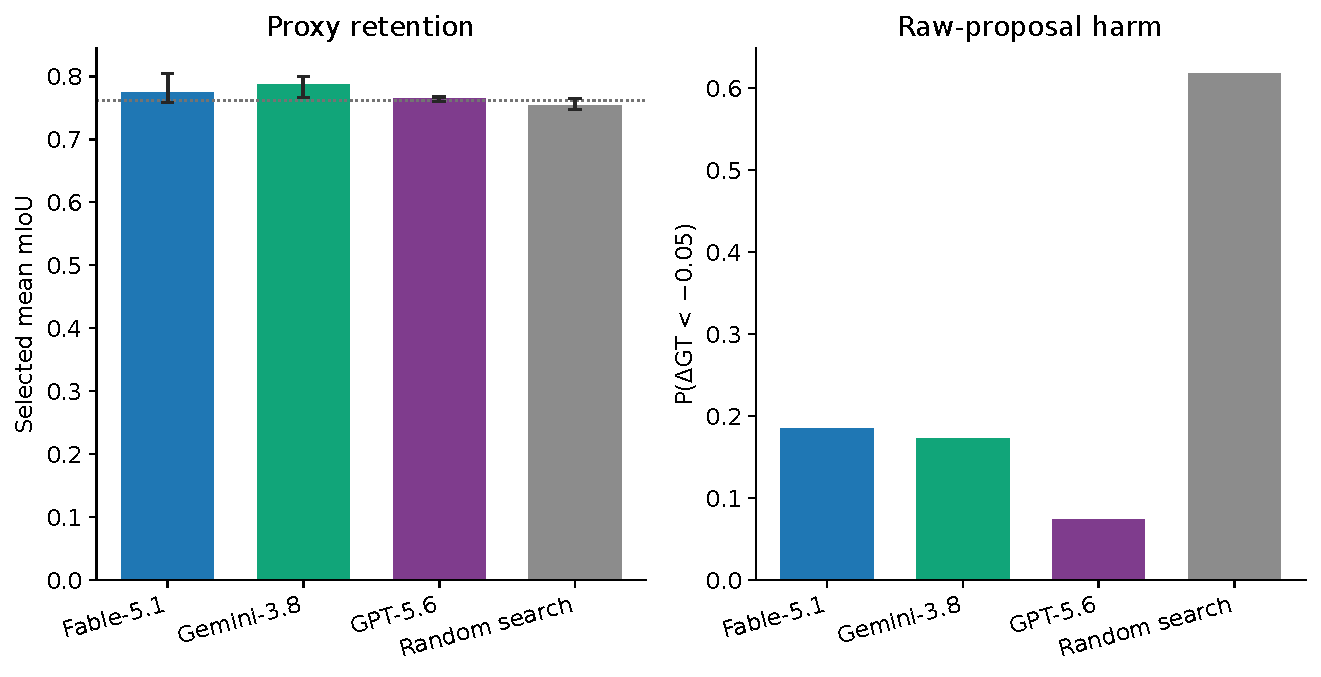
\includegraphics[width=0.92\textwidth]{figs/assume_random_comparison.pdf}
\end{hlbox}
\caption{\hl{Self-refinement under the shared selector. Selected GT mIoU is compared with the expert-reference start, and raw harmful-proposal rates characterise proposer risk before selection.}}
\label{fig:assume_random_comparison}
\end{figure*} 

\begin{table*}[t]
\caption{\hl{Self-refinement on 27 held-out family-specific references under the shared $0.01$ retention rule. Improved/unchanged/worsened counts use GT mIoU changes above $0.005$, within $\pm0.005$, and below $-0.005$.}}\label{tab:arm-compare}
{\small
\begin{tabular*}{\textwidth}{@{\extracolsep{\fill}} l c c c c c @{}}
\toprule
Arm & Selected mean & Mean $\Delta$ & 95\% CI for mean gain & Up/same/down & Worst $\Delta$ \\
\midrule
Reference start & 0.762 & -- & -- & -- & -- \\
\rowcolor{yellow!25}GPT-5.6 & 0.765 & $+0.003$ & $[-0.002,\,0.005]$ & 3/22/2 & $-0.013$ \\
\rowcolor{yellow!25}Fable-5.1 & 0.774 & $+0.012$ & $[-0.004,\,0.042]$ & 4/20/3 & $-0.143$ \\
\rowcolor{yellow!25}Gemini-3.8 & 0.787 & $+0.025$ & $[0.005,\,0.037]$ & 7/14/6 & $-0.185$ \\
\rowcolor{yellow!25}Random search & 0.754 & $-0.008$ & $[-0.016,\,0.002]$ & 3/21/3 & $-0.129$ \\
\bottomrule
\end{tabular*}}
\end{table*}

\hl{The expert-reference configurations start at mean GT mIoU $0.762$. The shared proxy selector reaches $0.765$ for GPT-5.6, $0.774$ for Fable-5.1, and $0.787$ for Gemini-3.8, whereas adaptive-random reaches $0.754$ (Table~\ref{tab:arm-compare}; Fig.~\ref{fig:assume_random_comparison}). All three LLM arms therefore finish above the common start in mean accuracy, while random search finishes below it. Individual selections can still deteriorate. Before selection, the harmful-proposal rates are 0.07, 0.19, and 0.17 for GPT-5.6, Fable-5.1, and Gemini-3.8, compared with 0.62 for adaptive-random.}

\begin{table*}[t]
\caption{\hl{Concentration of selected gains by starting GT mIoU. The split at 0.7 is retrospective and is not an admission rule.}}\label{tab:gain-concentration}
\begin{tabular*}{\textwidth}{@{\extracolsep{\fill}} l c c c c @{}}
\toprule
Arm & Mean $\Delta$ (start $<0.7$) & Mean $\Delta$ (start $\geq0.7$) & Spearman(start,$\Delta$) & Leave-one-parent range \\
\midrule
\rowcolor{yellow!25}Fable-5.1 & $+0.078$ & $-0.006$ & $-0.252$ & 0.004--0.026 \\
\rowcolor{yellow!25}Gemini-3.8 & $+0.143$ & $-0.009$ & $-0.406$ & 0.017--0.029 \\
\rowcolor{yellow!25}GPT-5.6 & $+0.010$ & $+0.001$ & $-0.258$ & 0.001--0.004 \\
\rowcolor{yellow!25}Random search & $+0.001$ & $-0.011$ & $-0.252$ & $-0.010$--$-0.005$ \\
\bottomrule
\end{tabular*}
\end{table*}

\begin{figure*}[t]
\centering
\begin{hlbox}
\centering
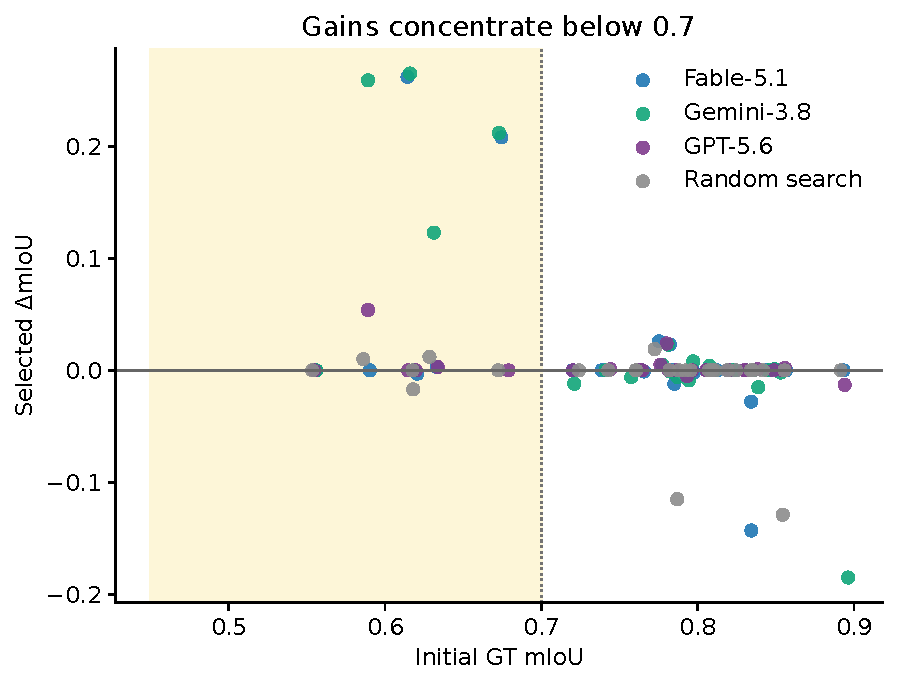
\includegraphics[width=0.92\textwidth]{figs/assume_gain_concentration.pdf}
\end{hlbox}
\caption{\hl{Selected gains concentrate on the six weaker starts below 0.7 GT mIoU; the 21 stronger starts are approximately flat or slightly negative.}}
\label{fig:assume_gain_concentration}
\end{figure*}

\hl{The aggregate means conceal where improvement occurs (Table~\ref{tab:gain-concentration}; Fig.~\ref{fig:assume_gain_concentration}). Fable-5.1 and Gemini-3.8 gain $0.078$ and $0.143$ on the six starts below 0.7, but change by $-0.006$ and $-0.009$ on the 21 stronger starts. GPT-5.6 is nearly flat in both groups, and random search is slightly negative overall. This concentration is retrospective; starting GT mIoU is not used for admission or selection.}

\subsection{\hl{External STSD control}}
\label{sec:stsd-control}

\hl{On the additional STSD subset, nine controlled proposals are evaluated from a fixed intermediate state with proxy score $0.5578$, zero assumed lines, and first-10 mIoU $0.7277$. Eight proposals are rejected and one angular adjustment is retained at proxy score $0.5664$, zero assumed lines, and first-10 mIoU $0.7276$. This is initial evidence from one external control without an STSD-specific expert reference, not a second panel benchmark; the complete audit is given in Appendix~\ref{app:stsd-control}.}



\subsection{Error analysis: block-identity shifts}
\label{sec:error-analysis}

\hl{Case 1-5 illustrates a blind spot. Its start has proxy score $0.610$. Fable-5.1 reaches score $0.636$ with GT mIoU $0.884$, and Gemini-3.8 reaches score $0.644$ with mIoU $0.888$: large accuracy changes produce only modest proxy movement.}

\hl{The K-block position anchors block identities around each ring. Incorrect K-block localisation can shift the label sequence while preserving geometric boundaries, fill, depth completeness, assumed-line count, and joint--boundary agreement. The proxy can therefore miss an important identity correction or select a geometrically coherent but mislabeled output. The largest losses in Table~\ref{tab:arm-compare} show the converse risk. More reliable K-block localisation or independent block-identity evidence is needed; a coherence metric derived from the same layout may remain insensitive to the error.}




% ══════════════════════════════════════════════════════════════════════════
\section{Discussion}\label{sec:discussion}
% ══════════════════════════════════════════════════════════════════════════

The results answer the research question of Section~\ref{sec:intro} in two parts. Intermediate metrics do carry accuracy information that survives transfer to \hl{held-out tunnel sections} and, less evenly, to unseen families. \hl{Proxy-based retention reduces losses relative to accepting proposals unconditionally, but selection errors can still reduce true accuracy. Final performance depends on both proposal quality and proxy accuracy.}

\subsection{Key findings}

\textbf{Fewer features transfer better.} The design principle of Section~\ref{sec:methods} was to select for transfer, not fit, and the ablation bears this out: \hl{adding six metrics to the compact four lowered LOFO $\rho$ from $0.754$ to $0.744$.} \hl{With 120 runs from three development subsets, a proxy that explains its own calibration set is not the goal; one that still orders runs on a family it has not seen is. The cost is coverage: the four retained features do not detect a block-identity shift.}

\textbf{Retention limits losses and can still select a worse output.} \hl{Proxy-based retention reduces losses relative to accepting proposals unconditionally, but selection errors can still reduce true accuracy. Final performance depends on both proposal quality and proxy accuracy.} \hl{Adaptive-random retention reaches $0.754$ from the $0.762$ start.} The same rule retains the losses in Table~\ref{tab:arm-compare}. The control compares proposal strategies under the same bounds, attempt budget, and retention rule; it does not isolate the use of pipeline evidence from differences in proposal size or parameter choice (Section~\ref{sec:agent-design}).

\textbf{What deployment would look like.} Each pipeline release still needs one expert reference per family and one calibration pass. From then on the frozen proxy supplies a label-free score that can be monitored over time and used as the selection signal inside the bounded self-refinement loop; three bounded attempts cost roughly 15 GPU-minutes. On this study's constructed reference--degraded pairs, a proxy threshold of $0.4$ (chosen retrospectively within the observed separation gap) flags all degradations and none of the references, but this does not by itself validate a deployment cutoff. Self-refinement is assisted, auditable reconfiguration against a strong engineering baseline, not autonomous inspection.

\subsection{Comparison with state-of-the-art}\label{sec:positioning}
\begin{table*}[t]
\caption{Positioning Proxy4Tun against representative tunnel-segmentation paradigms. The comparison concerns setup cost and deployment capability as well as accuracy. mIoU figures are \emph{not} measured under comparable settings: supervised and expert-tuned figures are taken from prior work under their original protocols, whereas Proxy4Tun figures are from this study (27 held-out family-specific references).}\label{tab:sota}
\begin{tabular*}{\textwidth}{@{\extracolsep{\fill}} l c c c l @{}}
\toprule
Method & \begin{tabular}[t]{@{}c@{}}Deep learning\\training\end{tabular} & \begin{tabular}[t]{@{}c@{}}Per-case\\tuning\end{tabular} & \begin{tabular}[t]{@{}c@{}}Deployment-label-free\\quality signal\end{tabular} & mIoU (setting) \\
\midrule
LiningNet/SparseUNet/SCF-Net/FA-ResNet & \checkmark & -- & -- & 0.83--0.90 \\
SAM4Tun & -- & Expert & -- & above 0.90 \\
\textbf{Proxy4Tun} (four-feature + LLM) & -- & \textbf{Auto} & \checkmark & \textbf{\hl{0.765--0.787}} \\
\bottomrule
\end{tabular*}
\end{table*}

Comparisons here concern operating points, not accuracy leaderboards (Table~\ref{tab:sota}). Supervised 3D models on Seg2Tunnel report strong in-distribution accuracy~\cite{lin2024seg2tunnel} but require per-point labels and provide no deployment-time accept/refine/flag gate. Expert-tuned SAM4Tun reaches high accuracy on curated rings~\cite{ye2025sam4tun}, but a fixed configuration emits no signal when it degrades. Relative to that static pipeline, Proxy4Tun adds an explicit quality signal and a bounded self-refinement loop. The only directly comparable contrast in this study is LLM-plus-proxy versus random-plus-proxy under the shared reference starts and selection rule. The mIoU gap to expert-tuned SAM4Tun in Table~\ref{tab:sota} is therefore not a like-for-like deficit: those figures come from curated rings with per-case expert tuning, whereas the Proxy4Tun figures are 27 \hl{held-out subsets} with three automated attempts each.

\subsection{Limitations}\label{sec:limitations}

Four limitations bound the claims. First, the evidence base is narrow: \hl{120 calibration runs come from three development subsets. Some held-out subsets come from the same parent tunnels; tunnels 1 and 4 are other tunnels in this collection.} Transfer is shown to \hl{held-out tunnel sections} within this collection, not to new projects or lining geometries, and the weak continuous-family LOFO result ($\rho=\hl{0.479}$) shows that even within-collection transfer is uneven. \hl{The single STSD subset is an external control, not a general external benchmark.} Second, \hl{the four features do not detect a block-identity shift from incorrect K-block localisation, so a higher proxy score can accompany lower GT accuracy, and the two largest LLM losses passed the selection rule for this reason.} Third, the degradations are constructed and the panel is small: \hl{the natural proposals arise from the same bounded refinement experiment rather than an independent deployment stream,} and with five parent tunnels the bootstrap intervals for GPT-5.6 and Fable-5.1 include zero, so their gains are descriptive. Fourth, the loop is one expert reference and three attempts; nothing here shows sustained improvement over longer horizons or without a reference to start from.


% ══════════════════════════════════════════════════════════════════════════
\section{Conclusions}\label{sec:conclusions}
% ══════════════════════════════════════════════════════════════════════════

This paper asked whether intermediate tunnel-segmentation metrics can estimate accuracy and guide parameter self-refinement on \hl{held-out tunnel sections} without new GT labels. Proxy4Tun answers with a four-feature Ridge proxy calibrated from 120 runs around one expert reference per lining family, selected for cross-family transfer rather than fit, and frozen before any held-out scan is scored.

\begin{itemize}
\item The metrics carry transferable accuracy information. Three structure-coherence features and one preprocessing-quality feature reach Spearman $\hl{0.789}$ on 54 held-out runs and order every reference above its degraded partner; adding more features hurt transfer.
\item \hl{From a} $0.762$ \hl{baseline, LLM proposals under the selection rule reach} $0.765$\hl{--}$0.787$\hl{, while adaptive-random proposals under the same rule reach} $0.754$\hl{. Proxy-based retention reduces losses relative to accepting proposals unconditionally, but selection errors can still reduce true accuracy.}
\item \hl{Final performance depends on both proposal quality and proxy accuracy.}
\end{itemize}

\hl{The principal remaining limit is a block-identity shift: the four features can approve an output whose K-block localisation is wrong. Future work should add reliable K-block localisation or independent block-identity evidence, test the loop on naturally degraded runs and on tunnels outside this collection, and examine whether the proxy can guide refinement without an expert reference to start from.} Until then, Proxy4Tun is a label-free assessment and assisted-reconfiguration tool, not an autonomous inspector.

% ══════════════════════════════════════════════════════════════════════════
% Data availability, declarations, etc.
% ══════════════════════════════════════════════════════════════════════════

\section*{Data availability}

The source code, parameter snapshots, exploration-trial tables, and evaluation scripts will be released upon publication. The Seg2Tunnel dataset is publicly available~\cite{lin2024seg2tunnel}.

\section*{Declaration of competing interest}

The authors declare that they have no known competing financial interests or personal relationships that could have appeared to influence the work reported in this paper.

\section*{Declaration of generative AI use}

During this study, LLM agents (GPT-5.6, Fable-5.1, and Gemini-3.8) were evaluated as proposal mechanisms in the self-refinement loop, together with a random-search control under the same proxy-based selection rule. LLMs were also used for language editing and for improving manuscript structure. The authors reviewed and edited all content and take full responsibility for the content of the publication.

% ══════════════════════════════════════════════════════════════════════════
% Bibliography
% ══════════════════════════════════════════════════════════════════════════

% Natbib requires a BibTeX style; without it, citations stay as “?”
% NOTE: \balance can cause column-balancing artefacts in the reference list (e.g.,
% lines slipping into the footer area) with this class. Keep it off for the bibliography.
%\balance
\bibliographystyle{model1-num-names}
\bibliography{references}


% ══════════════════════════════════════════════════════════════════════════
% Appendix
% ══════════════════════════════════════════════════════════════════════════

\appendix

\section{Pipeline anchor parameters}\label{app:anchor-parameter}

This appendix summarises the expert-tuned \emph{anchor} parameter profiles used to warm-start the segmentation pipeline for each lining family (staggered, continuous, complex). Table~\ref{tab:anchor-params} lists the fixed stage algorithms and the corresponding family-specific parameter values that define the reference configurations used throughout the study.

\begin{table*}[t]
\caption{Pipeline anchor parameters: expert-tuned, family-specific anchor parameter profiles of the segmentation pipeline.}\label{tab:anchor-params}
\begin{tabular*}{\textwidth}{@{\extracolsep{\fill}} l l p{0.30\textwidth} l @{}}
\toprule
Stage & Parameter & Description & Staggered / Continuous / Complex \\
\midrule
Unfolding & \texttt{diameter} & Cylindrical scale. & 5.5 / 5.9 / 7.5\,m \\
Unfolding & \texttt{slice\_spacing\_factor} & Slice spacing (ring width). & 1.2 / 1.2 / 1.8\,m \\
Unfolding & \texttt{polynomial\_degree} & Centreline fit degree. & 3 / 2 / 2 \\
Unfolding & \texttt{residual\_recentre} & Per-bin frame recentring. & off / on / on \\
\midrule
Denoising & \texttt{mask\_r\_low} & Inner radial gate. & 2.33 / 2.85 / 3.65\,m \\
Denoising & \texttt{mask\_r\_high} & Outer radial gate. & 2.78 / 3.0 / 3.9\,m \\
Denoising & \texttt{y\_step} & Angular bin width. & 0.4 / 0.5 / 0.1\,m \\
Denoising & \texttt{z\_step} & Radial histogram bin width. & 0.005 / 0.001 / 0.001\,m \\
Denoising & \texttt{grad\_threshold} & Outer-edge gradient threshold. & 0.15 / 0.2 / 0.2 \\
Denoising & \texttt{smoothing\_window\_size} & Cutoff-curve smoothing window. & 5 / 3 / 3 \\
Denoising & \texttt{smoothing\_offset} & Post-smoothing cutoff bias. & $-$0.002 / $-$0.003 / $-$0.005\,m \\
Denoising & \texttt{default\_cutoff\_z} & Fallback radial cutoff. & 2.75 / 2.85 / 3.65\,m \\
\midrule
Enhancing & \texttt{upsampling\_stage1} & Stage-1 upsampling spacing. & 0.06 / 0.08 / 0.09\,m \\
Enhancing & \texttt{upsampling\_stage2} & Stage-2 upsampling spacing. & 0.03 / 0.04 / 0.045\,m \\
Enhancing & \texttt{upsampling\_stage3} & Stage-3 upsampling spacing. & 0.015 / 0.02 / 0.0225\,m \\
Enhancing & \texttt{curvature\_threshold} & Panel--joint curvature threshold. & 0.005 / 0.0005 / 0.0005 \\
Enhancing & \texttt{depth\_threshold\_low} & Lower interpolation depth tolerance. & 0.005 / 0.01 / 0.0065\,m \\
Enhancing & \texttt{depth\_threshold\_high} & Upper interpolation depth tolerance. & 0.015 / 0.01 / 0.013\,m \\
Enhancing & \texttt{inter\_radius} & Interpolation neighbour radius. & 0.03 / 0.06 / 0.06\,m \\
Enhancing & \texttt{n\_segment\_start/end} & Interpolated ring-index window. & 0--5 / 2--8 / 5--14 \\
Enhancing & \texttt{ring\_spacing\_factor} & Nominal ring width. & 1.2 / 1.2 / 1.8\,m \\
\midrule
Detecting & \texttt{binary\_threshold} & Depth-map binarisation level. & 125 / 127 / 125 \\
Detecting & \texttt{hough\_thresh\_obliq} & Oblique joint-line vote threshold. & 65 / 30 / 35 \\
Detecting & \texttt{hough\_thresh\_horiz} & Horizontal joint-line vote threshold. & 65 / 30 / 35 \\
Detecting & \texttt{hough\_thresh\_vert} & Ring-boundary vote threshold. & 600 / 1500 / 5000 \\
Detecting & \texttt{minLineLength\_obliq} & Minimum oblique line length. & 100 / 40 /  80\,px \\
Detecting & \texttt{minLineLength\_horiz} & Minimum horizontal line length. & 100 / 50 /  80\,px \\
Detecting & \texttt{maxLineGap\_obliq} & Oblique line-merging gap limit. & 45 / 30 /  60\,px \\
Detecting & \texttt{maxLineGap\_horiz} & Horizontal line-merging gap limit. & 10 / 10 /  15\,px \\
Detecting & \texttt{angle\_range\_oblique} & Oblique-joint angle band. & $\pm$[6, 9] / $\pm$[4, 10] / $\pm$[5, 10]$^{\circ}$ \\
\midrule
Segmenting & \texttt{segment\_per\_ring} & Segments per lining ring. & 6 / 6 / 7 \\
Segmenting & \texttt{segment\_order} & Circumferential segment order. & \begin{tabular}[t]{@{}l@{}}K,B1,A1--A3,B2 /\\K,B2,A3--A1,B1 /\\K,B1,A1--A4,B2\end{tabular} \\
Segmenting & \texttt{segment\_width} & Nominal segment width. & 1200 / 1200 / 1800\,mm \\
Segmenting & \texttt{K\_height} & Key-segment arc height. & 1079.9 / 823.8 / 1227.0\,mm \\
Segmenting & \texttt{AB\_height} & Standard-segment arc height. & 3239.8 / 3346.8 / 3726.9\,mm \\
Segmenting & \texttt{angle} & Oblique K-joint inclination. & 7.52 / 6.12 / 9.8$^{\circ}$ \\
Segmenting & \texttt{processing.y\_bounds} & Valid panorama band. & 3800--13300 / 4500--14000 / 4200--13100\,px \\
\bottomrule
\end{tabular*}
\end{table*}

\section{Bayesian exploration configuration}\label{app:bo-config}

Table~\ref{tab:bo-config} records the frozen design-time exploration settings
used to generate the 120 calibration trials. Accepted trials are exactly
$N_0{=}32$ Sobol $+\,N_{\mathrm{GP}}{=}8$ GP-uncertainty acquisitions per family
(40 valid trials each).

\begin{table*}[t]
\caption{Design-time Bayesian exploration configuration (frozen snapshot).}\label{tab:bo-config}
\begin{tabular*}{\textwidth}{@{\extracolsep{\fill}} l l @{}}
\toprule
Setting & Value \\
\midrule
Target accepted trials / family & $N{=}40$ ($N_0{=}32$ Sobol, $N_{\mathrm{GP}}{=}8$ accepted GP) \\
Sobol & Scrambled QMC in the unit cube \\
GP kernel & Mat\'{e}rn $\nu{=}2.5$ $+$ white noise; \texttt{normalize\_y=True} \\
Length-scale bounds & $(10^{-2},10^{2})$ per dimension; noise $(10^{-6},10^{-1})$ \\
GP optimiser & \texttt{GaussianProcessRegressor}, $n_{\mathrm{restarts\_optimizer}}{=}3$ \\
Acquisition & Maximise predictive std over random candidate pool $\mathcal{P}_{\mathrm{BO}}$ of size $2048$ \\
Failure / top-up rule & Status not ok or required features incomplete $\Rightarrow$ exclude; continue until accepted targets met \\
\bottomrule
\end{tabular*}
\end{table*}

\section{Per-family search-space bounds}\label{app:search-bounds}

This appendix reports the full bounded per-family search spaces $B$ used for Bayesian exploration. Table~\ref{tab:bo-bounds} enumerates every optimised parameter and its allowable range (or discrete set) for each family reference case, defining the constraints enforced during the frozen 120-trial campaign.

\begin{table*}[t]
\caption{Complete per-family search-space bounds $B$ for the frozen 120-trial campaign.}\label{tab:bo-bounds}
{\small
\begin{tabular*}{\textwidth}{@{\extracolsep{\fill}} llp{0.28\textwidth} @{}}
\toprule
Family (case) & Parameter & Bounds \\
\midrule
Staggered (2-1) & \texttt{unfolding.ransac\_threshold} & $[0.8,1.2]$ \\
 & \texttt{unfolding.slice\_spacing\_factor} & $[1.05,1.35]$ \\
 & \texttt{unfolding.polynomial\_degree} & $\{2,3\}$ \\
 & \texttt{unfolding.random\_seed} & $\{0,\ldots,7\}$ \\
 & \texttt{denoising.mask\_r\_low} & $[2.2,2.5]$ \\
 & \texttt{denoising.mask\_r\_high} & $[2.7,2.9]$ \\
 & \texttt{denoising.z\_step} & $[0.001,0.008]$ \\
 & \texttt{denoising.grad\_threshold} & $[0.1,0.25]$ \\
 & \texttt{enhancing.curvature\_threshold} & $[3{\times}10^{-4},8{\times}10^{-3}]$ \\
 & \texttt{enhancing.inter\_radius} & $[0.02,0.08]$ \\
 & \texttt{detecting.binary\_threshold} & $[100,160]$ \\
 & \texttt{detecting.hough\_threshold\_oblique} & $[40,90]$ \\
 & \texttt{detecting.hough\_threshold\_horizontal} & $[40,90]$ \\
 & \texttt{detecting.hough\_threshold\_vertical} & $[400,800]$ \\
 & \texttt{detecting.maxLineGap\_oblique} & $[20,80]$ \\
 & \texttt{sam.y\_bounds\_lower} & $[3600,4400]$ \\
\addlinespace
Continuous (3-1) & \texttt{unfolding.ransac\_threshold} & $[0.8,1.2]$ \\
 & \texttt{unfolding.slice\_spacing\_factor} & $[1.05,1.35]$ \\
 & \texttt{unfolding.polynomial\_degree} & $\{2,3\}$ \\
 & \texttt{unfolding.random\_seed} & $\{0,\ldots,7\}$ \\
 & \texttt{denoising.mask\_r\_low} & $[2.7,3.0]$ \\
 & \texttt{denoising.mask\_r\_high} & $[2.9,3.15]$ \\
 & \texttt{denoising.mask\_theta\_low} & $[1.0,2.5]$ \\
 & \texttt{denoising.mask\_theta\_high} & $[15,19]$ \\
 & \texttt{enhancing.curvature\_threshold} & $[2{\times}10^{-4},2{\times}10^{-3}]$ \\
 & \texttt{detecting.binary\_threshold} & $[100,160]$ \\
 & \texttt{detecting.hough\_threshold\_oblique} & $[20,60]$ \\
 & \texttt{detecting.hough\_threshold\_horizontal} & $[20,60]$ \\
 & \texttt{detecting.hough\_threshold\_vertical} & $[800,2500]$ \\
 & \texttt{detecting.maxLineGap\_oblique} & $[10,60]$ \\
 & \texttt{detecting.pattern\_tolerance} & $[5,20]$ \\
 & \texttt{detecting.uniform\_k\_snap} & $\{\mathrm{off},\mathrm{on}\}$ \\
 & \texttt{sam.segment\_width} & $[1000,1400]$ \\
 & \texttt{sam.K\_height} & $[700,1000]$ \\
 & \texttt{sam.angle} & $[4,9]$ \\
\addlinespace
Complex (5-1) & \texttt{unfolding.ransac\_threshold} & $[0.8,1.2]$ \\
 & \texttt{unfolding.slice\_spacing\_factor} & $[1.6,2.0]$ \\
 & \texttt{unfolding.polynomial\_degree} & $\{2,3\}$ \\
 & \texttt{unfolding.random\_seed} & $\{0,\ldots,7\}$ \\
 & \texttt{denoising.mask\_r\_low} & $[3.5,3.8]$ \\
 & \texttt{denoising.mask\_r\_high} & $[3.75,4.05]$ \\
 & \texttt{enhancing.curvature\_threshold} & $[2{\times}10^{-4},2{\times}10^{-3}]$ \\
 & \texttt{detecting.binary\_threshold} & $[100,160]$ \\
 & \texttt{detecting.hough\_threshold\_oblique} & $[25,70]$ \\
 & \texttt{detecting.hough\_threshold\_horizontal} & $[25,70]$ \\
 & \texttt{detecting.hough\_threshold\_vertical} & $[800,5000]$ \\
 & \texttt{detecting.maxLineGap\_oblique} & $[30,80]$ \\
 & \texttt{detecting.maxLineGap\_horizontal} & $[5,30]$ \\
 & \texttt{detecting.pattern\_tolerance} & $[5,20]$ \\
 & \texttt{sam.segment\_width} & $[1500,2100]$ \\
 & \texttt{sam.K\_height} & $[1000,1500]$ \\
 & \texttt{sam.angle} & $[7,12]$ \\
\bottomrule
\end{tabular*}}
\end{table*}


\section{Tunnel ontology structure}\label{app:ontology}

The reflective agent consults a staged SAM4Tun ontology that encodes pipeline
artifacts, per-stage parameters and quality metrics, failure modes, diagnostic
rules, remediation actions, and inter-stage dependencies. The top-level schema
is summarised below:
We omit the complete YAML and show only the structure plus one representative
stage example.

\begin{lstlisting}[caption={Ontology top-level keys and stage inventory.},label={lst:ontology-structure}]
meta                  # version, domain, coordinate systems
artifacts             # data objects (cloud, depth map, masks, ...)
stages[]              # pipeline stages (unfolding through segmentation):
  stage_1_centreline
  stage_2_denoise
  stage_3_upsample
  stage_4_detection
  stage_5_segmentation
inter_stage_dependencies[]   # upstream cause -> defer local retune
diagnostic_rules[]           # metric patterns -> failure modes
remediation_actions[]        # bounded parameter changes
agent_interface              # {state, diagnosis, proposal}
\end{lstlisting}

\begin{lstlisting}[caption={Example ontology stage: radial denoising failure modes.},label={lst:ontology-example}]
- id: stage_2_denoise
  name: Local density-difference-based denoising
  quality_metrics:
    - id: m_retained_ratio
      healthy: "lining kept; background removed"
    - id: m_bg_leakage
      healthy: "near zero"
  failure_modes:
    - id: f_over_gate
      name: Radial gate too tight
      symptom: "lining removed; holes in later depth map"
    - id: f_under_gate
      name: Radial gate too loose
      symptom: "rails/tube/noise retained downstream"
\end{lstlisting}

\section{Agent prompt structure}\label{app:prompt}

Each reflection round issues a single bounded JSON overlay. The model-facing
prompt is assembled from a fixed skeleton (role, isolation rules, current
state, GT-blind intrinsics, four-feature proxy scores, allowed artifact images,
family parameter bounds, and the required output schema). Listing~\ref{lst:prompt-skeleton}
summarises the skeleton; Listing~\ref{lst:prompt-example} gives one example
proposal. GT mIoU and evaluation directories are never included.

\begin{lstlisting}[caption={Agent-prompt skeleton (per round).},label=lst:prompt-skeleton]
Role: reflective parameter agent for SAM4Tun
Allowed context:
  - family reference priors / warm-start parameters
  - GT-blind intrinsics and four-feature proxy scores
  - stage artifacts (depth map, detections, SAM masks)
  - ontology + bounded family search space
State: subset, family, reference proxy, operating band
Task: diagnose failure mode; propose ONE overlay within bounds
Output JSON keys (required):
  observation, failure_mode, rationale, overlay
\end{lstlisting}

\begin{lstlisting}[caption={Example JSON proposal returned by the agent.},label=lst:prompt-example]
{
  "observation": "Centreline residual is high; unroll shows asymmetric voids.",
  "failure_mode": "f_curve_underfit (under-fit centre curve)",
  "rationale": "Raise polynomial degree and tighten RANSAC before retuning SAM.",
  "overlay": {
    "unfolding": {
      "polynomial_degree": 3,
      "ransac_threshold": 0.9
    }
  }
}
\end{lstlisting}

\section{Random-search control}\label{app:random-search}

The random-search control samples sparse overlays. Let $k$ be the number of parameters changed in a round. We draw $k$ from a frozen empirical distribution estimated from an earlier LLM pilot campaign (198 proposals across three LLM arms), then sample $k$ distinct parameters uniformly (without replacement) from the bounded search space and sample each chosen parameter value uniformly within its family-specific bounds. That pilot distribution does not match the present LLM proposals: this experiment records a mean of $8.64$ changed parameters for random against $4.11$--$7.35$ for the LLM arms. Unfolding parameters are eligible only when the start's centreline residual exceeds 10\,cm, matching the constraint applied to LLM arms. Parameter identities and values are otherwise random; the overlay is applied to the retained configuration, and retention uses the proxy score. The distribution and seed were frozen before any LLM attempt in this study, so the control cannot track the LLM runs it is compared with.

\begin{hlbox}
\noindent\textbf{Frozen sampling design.} Seed base $20260915$; the generator for case index $i$ and round $r$ is seeded with $20260915+1000\,i+r$. Change-count probabilities $\Pr(k)$, $k=1,\ldots,15$:
\begin{center}
\small
\setlength{\tabcolsep}{3.5pt}
\begin{tabular}{@{}l cccccccc@{}}
\toprule
$k$ & 1 & 2 & 3 & 4 & 5 & 6 & 7 & 8 \\
$\Pr(k)$ & .036 & .005 & .025 & .030 & .046 & .061 & .066 & .051 \\
\midrule
$k$ & 9 & 10 & 11 & 12 & 13 & 14 & 15 & \\
$\Pr(k)$ & .076 & .071 & .157 & .188 & .107 & .076 & .005 & \\
\bottomrule
\end{tabular}
\end{center}
A draw of $k$ larger than the number of eligible parameters is clipped to that number.
\end{hlbox}

\section{Predefined parameter perturbations}\label{app:degradation}

Each held-out subset is paired with one family-specific overlay taken from the lowest-GT-mIoU valid calibration trial of that family's development subset. Unfolding keys are dropped so the perturbation does not change the centreline; the remaining stage-2 to stage-5 keys are applied to the family reference. The three overlays were frozen before any held-out scoring. All 54 runs completed, so no perturbation was replaced.

\begin{hlbox}
\small
\noindent\textbf{Staggered} (source 2-1/s017, source GT mIoU $0.032$).
\texttt{mask\_r\_low}$=2.207$,
\texttt{mask\_r\_high}$=2.741$,
\texttt{z\_step}$=0.00633$,
\texttt{grad\_threshold}$=0.183$,
\texttt{curvature\_threshold}$=7.14\times10^{-4}$,
\texttt{inter\_radius}$=0.0353$,
\texttt{binary\_threshold}$=125$,
\texttt{hough\_threshold\_oblique}$=46$,
\texttt{hough\_threshold\_horizontal}$=60$,
\texttt{hough\_threshold\_vertical}$=520$,
\texttt{maxLineGap\_oblique}$=36$,
\texttt{processing.y\_bounds}$=[4003,13100]$.

\medskip
\noindent\textbf{Continuous} (source 3-1/s030, source GT mIoU $0.042$).
\texttt{mask\_r\_low}$=2.756$,
\texttt{mask\_r\_high}$=2.906$,
\texttt{mask\_theta\_low}$=2.063$,
\texttt{mask\_theta\_high}$=18.79$,
\texttt{curvature\_threshold}$=1.55\times10^{-3}$,
\texttt{binary\_threshold}$=106$,
\texttt{hough\_threshold\_oblique}$=32$,
\texttt{hough\_threshold\_horizontal}$=37$,
\texttt{hough\_threshold\_vertical}$=2457$,
\texttt{pattern\_tolerance}$=13$,
\texttt{segment\_width}$=1315$,
\texttt{K\_height}$=944$,
\texttt{angle}$=5.56^{\circ}$.

\medskip
\noindent\textbf{Complex} (source 5-1/g001, source GT mIoU $0.036$).
\texttt{mask\_r\_low}$=3.776$,
\texttt{mask\_r\_high}$=3.961$,
\texttt{curvature\_threshold}$=2.42\times10^{-4}$,
\texttt{binary\_threshold}$=159$,
\texttt{hough\_threshold\_oblique}$=33$,
\texttt{hough\_threshold\_horizontal}$=26$,
\texttt{hough\_threshold\_vertical}$=4596$,
\texttt{maxLineGap\_oblique}$=40$,
\texttt{maxLineGap\_horizontal}$=22$,
\texttt{pattern\_tolerance}$=15$,
\texttt{segment\_width}$=1847$,
\texttt{K\_height}$=1014$,
\texttt{angle}$=8.35^{\circ}$.
\end{hlbox}

\section{\hl{Assumed-line proxy parameters}}\label{app:assume-proxy}

\hl{Table~\ref{tab:assume-proxy-parameters} gives the frozen scaler and coefficients used for the assumed-line result analysis. The intercept is $0.3588667$ and the ridge penalty is $\alpha=5.623413$.}

\begin{table*}[t]
\caption{\hl{Frozen assumed-line proxy parameters.}}\label{tab:assume-proxy-parameters}
\centering
\begin{tabular}{lrrr}
\toprule
Feature & Calibration mean & Calibration SD & Coefficient \\
\midrule
\rowcolor{yellow!25}Correspondence F1@15 & 0.1652637 & 0.1517009 & $+0.0884432$ \\
\rowcolor{yellow!25}SAM fill rate & 0.4568573 & 0.2836379 & $+0.1058000$ \\
\rowcolor{yellow!25}Assumed-line count & 4.5916667 & 3.6594531 & $-0.0215581$ \\
\rowcolor{yellow!25}Missing-depth rate & 0.4074803 & 0.3033190 & $-0.0339974$ \\
\bottomrule
\end{tabular}
\end{table*}

\section{\hl{STSD external-control audit}}\label{app:stsd-control}

\hl{The fixed starting context has proxy score $0.5578$, zero assumed lines, and first-10 mIoU $0.7277$. The nine controlled follow-up proposals are listed in Table~\ref{tab:stsd-control} and visualised in Fig.~\ref{fig:assume-stsd-control}.}

\begin{table*}[t]
\caption{\hl{STSD control from the fixed intermediate state.}}\label{tab:stsd-control}
{\footnotesize
\begin{tabular*}{\textwidth}{@{\extracolsep{\fill}} l c l l c c c @{}}
\toprule
Arm & Round & Proposed update & Outcome & Proxy & Assumed lines & mIoU$_{10}$ \\
\midrule
\rowcolor{yellow!25}GPT-5.6 & 1 & \texttt{prompt\_logic=notebook\_12} & Rejected & 0.5578 & 0 & 0.7277 \\
\rowcolor{yellow!25}GPT-5.6 & 2 & \texttt{AB\_height=3220} & Rejected & 0.3601 & 0 & 0.7147 \\
\rowcolor{yellow!25}GPT-5.6 & 3 & \texttt{y\_bounds=[3000,12900]} & Rejected & 0.5326 & 0 & 0.7285 \\
\rowcolor{yellow!25}Gemini-3.8 & 1 & \texttt{prompt\_logic=t12\_pattern} & Rejected & 0.5218 & 0 & 0.6018 \\
\rowcolor{yellow!25}Gemini-3.8 & 2 & \texttt{y\_bounds=[2800,13100]} & Rejected & 0.5311 & 0 & 0.7292 \\
\rowcolor{yellow!25}Gemini-3.8 & 3 & \texttt{key\_pair\_max\_sep\_px=300} & Rejected & 0.5578 & 0 & 0.7277 \\
\rowcolor{yellow!25}Fable-5.1 & 1 & \texttt{padding=250} & Rejected & 0.5280 & 0 & 0.7293 \\
\rowcolor{yellow!25}Fable-5.1 & 2 & \texttt{y\_bounds=[2800,13100]} & Rejected & 0.5311 & 0 & 0.7292 \\
\rowcolor{yellow!25}Fable-5.1 & 3 & \texttt{angle=8.0} & Retained & 0.5664 & 0 & 0.7276 \\
\bottomrule
\end{tabular*}}
\end{table*}

\begin{figure*}[t]
\centering
\begin{hlbox}
\centering
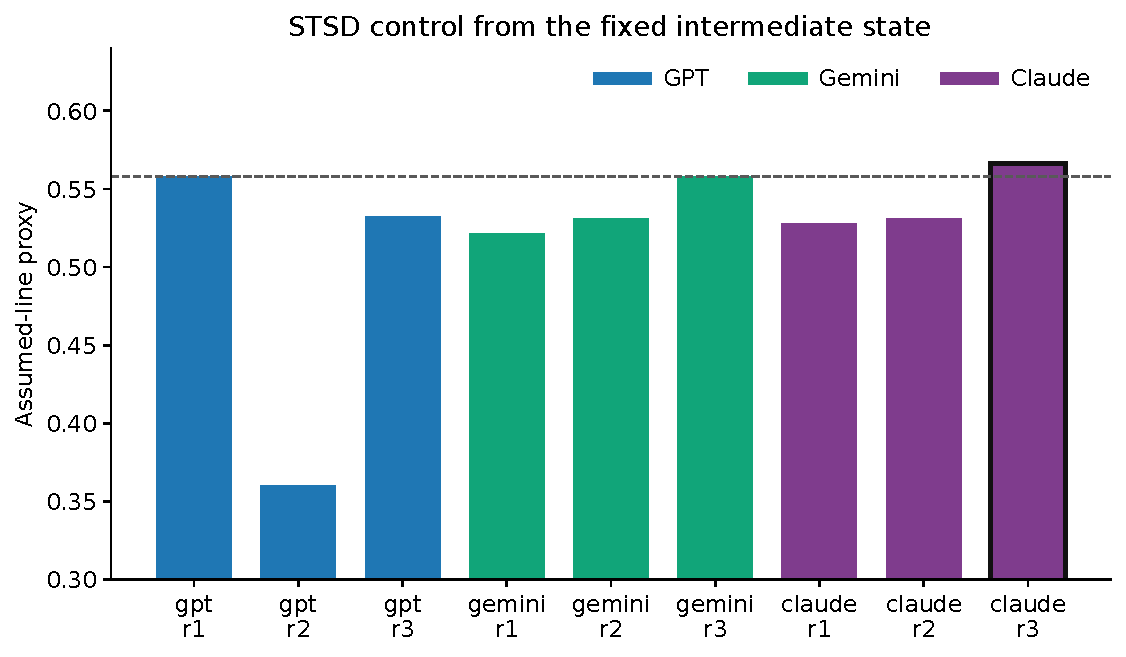
\includegraphics[width=0.92\textwidth]{figs/assume_stsd_control.pdf}
\end{hlbox}
\caption{\hl{Assumed-line proxy, first-10 mIoU, and assumed-line outcomes for the nine-proposal STSD control.}}
\label{fig:assume-stsd-control}
\end{figure*}

\section{Full-panel selection audit}\label{app:poc-selection}

Table~\ref{tab:panel-audit} summarises all 27 held-out family-specific references and the selected offline mIoU under each proposal arm. Starts are the family-specific reference configurations. Selected values follow the shared proxy selector with a retention margin: a candidate replaces the retained output only if its proxy score exceeds the retained score by more than $0.01$.

\begin{table*}[t]
\caption{Merged 27-case panel: reference start and selected GT mIoU by arm.}\label{tab:panel-audit}
{\footnotesize
\begin{tabular*}{\textwidth}{@{\extracolsep{\fill}} l l c cccc @{}}
\toprule
Subset & Family & Start & GPT-5.6 & Fable-5.1 & Gemini-3.8 & Random \\
\midrule
1-1 & staggered & 0.784 & 0.784 & 0.784 & 0.783 & 0.784 \\
1-2 & staggered & 0.809 & 0.809 & 0.809 & 0.809 & 0.809 \\
1-3 & staggered & 0.827 & 0.827 & 0.827 & 0.827 & 0.827 \\
\rowcolor{yellow!25}1-4 & staggered & 0.853 & 0.855 & 0.853 & 0.851 & 0.853 \\
1-5 & staggered & 0.676 & 0.676 & 0.884 & 0.888 & 0.676 \\
2-2 & staggered & 0.615 & 0.615 & 0.877 & 0.880 & 0.615 \\
\rowcolor{yellow!25}2-3 & staggered & 0.795 & 0.790 & 0.793 & 0.803 & 0.795 \\
2-4 & staggered & 0.835 & 0.835 & 0.807 & 0.835 & 0.835 \\
2-5 & staggered & 0.893 & 0.880 & 0.893 & 0.708 & 0.893 \\
3-2 & continuous & 0.631 & 0.634 & 0.634 & 0.754 & 0.643 \\
\rowcolor{yellow!25}3-3 & continuous & 0.808 & 0.808 & 0.808 & 0.812 & 0.808 \\
3-4 & continuous & 0.622 & 0.622 & 0.619 & 0.622 & 0.605 \\
3-5 & continuous & 0.588 & 0.642 & 0.588 & 0.847 & 0.598 \\
3-6 & continuous & 0.836 & 0.837 & 0.693 & 0.821 & 0.836 \\
3-7 & continuous & 0.845 & 0.845 & 0.845 & 0.845 & 0.786 \\
3-8 & continuous & 0.723 & 0.723 & 0.723 & 0.711 & 0.630 \\
3-9 & continuous & 0.820 & 0.820 & 0.820 & 0.820 & 0.820 \\
\rowcolor{yellow!25}3-10 & continuous & 0.853 & 0.853 & 0.854 & 0.854 & 0.724 \\
\rowcolor{yellow!25}4-1 & complex & 0.741 & 0.742 & 0.741 & 0.741 & 0.741 \\
4-2 & complex & 0.787 & 0.787 & 0.775 & 0.781 & 0.787 \\
4-3 & complex & 0.554 & 0.554 & 0.554 & 0.554 & 0.554 \\
4-4 & complex & 0.784 & 0.808 & 0.807 & 0.807 & 0.669 \\
4-5 & complex & 0.808 & 0.808 & 0.808 & 0.808 & 0.808 \\
5-2 & complex & 0.793 & 0.793 & 0.793 & 0.784 & 0.793 \\
5-3 & complex & 0.762 & 0.762 & 0.761 & 0.762 & 0.762 \\
5-4 & complex & 0.760 & 0.760 & 0.760 & 0.754 & 0.760 \\
5-5 & complex & 0.775 & 0.780 & 0.801 & 0.780 & 0.794 \\
\midrule
\rowcolor{yellow!25}Mean & -- & 0.762 & 0.765 & 0.774 & 0.787 & 0.754 \\
\bottomrule
\end{tabular*}}
\end{table*}

\end{document}